\documentclass[14pt,a4paper,final,russian]{report}
\usepackage[LCY]{fontenc}
\usepackage[utf8]{inputenc}
\usepackage[intlimits]{amsmath}
\usepackage{nccmath}
\usepackage{graphicx}
\graphicspath{{chapter_1/paragraph_1/img/}{chapter_1/paragraph_4/img/}{chapter_2/paragraph_1/img/}{chapter_3/paragraph_1/img/}{chapter_3/paragraph_3/img/}{appendix/img/}}
\usepackage[russian]{babel}
\usepackage{amssymb}
\usepackage{amsthm}
\usepackage{cite}
\usepackage{geometry} % Меняем поля страницы
\geometry{left=30mm}% левое поле
\geometry{right=10mm}% правое поле
\geometry{top=20mm}% верхнее поле
\geometry{bottom=20mm}% нижнее поле
% установка полуторного интервала
\usepackage{setspace}  
\onehalfspacing

\usepackage{fancyhdr}
\pagestyle{fancy}
\fancyhf{} % clear all header and footer fields
\fancyhead[C]{\thepage}
\renewcommand{\headrulewidth}{0pt}
\renewcommand{\footrulewidth}{0pt}
%  нумерация сверху
\fancypagestyle{plain}{%
	\fancyhf{} % clear all header and footer fields
	\fancyhead[C]{\thepage}
	\renewcommand{\headrulewidth}{0pt}
	\renewcommand{\footrulewidth}{0pt}}

\usepackage{titlesec}
\usepackage{needspace}
% переопределение главы
\titleformat{\chapter}[block]
{\filcenter}{\thechapter}{1em}{\MakeUppercase}{}
\titlespacing*{\chapter}{-25pt}{0pt}{*4}

%переопределение параграфа
\titleformat{\section}
{}{\thesection}{1em}{}
\titlespacing*{\section}{\parindent}{*4}{*4}


%\titleformat{\section}
%{\needspace{1in}\Large\bfseries}{\thesection}{1em}{}



\newenvironment{comment}{}{}
\renewcommand{\theenumi}{\arabic{enumi}}% Меняем везде перечисления на цифра.цифра
\renewcommand{\baselinestretch}{1}

\newenvironment{mpmatrix}{\begin{medsize}\begin{pmatrix}}%
{\end{pmatrix}\end{medsize}}%

\newtheorem{theorem}{Теорема}
\newcommand{\thrm}[1]{\begin{theorem}#1.1\end{theorem}}
\numberwithin{theorem}{chapter}

\newtheorem{lemma}{Лемма}
\newcommand{\lem}[1]{\begin{lemma}#1.1\end{lemma}}
\numberwithin{lemma}{chapter}

\newtheorem{consectary}{Следствие}
\newcommand{\cnsct}[1]{\begin{consectary}#1.1\end{consectary}}
\numberwithin{consectary}{chapter}

\newtheorem{pointout}{Замечание}
\newcommand{\pntout}[1]{\begin{pointout}#1.1\end{pointout}}
\numberwithin{pointout}{chapter}

\newtheorem{definition}{Определение} 
\newcommand{\defn}[1]{\begin{definition}#1.1\end{definition}}
\numberwithin{definition}{chapter}



\begin{document}
	
	
	% установка размера шрифта для всего документа
	\fontsize{14pt}{18pt}\selectfont
	\pretolerance10000
	\thispagestyle{empty}
\centerline{ФЕДЕРАЛЬНОЕ ГОСУДАРСТВЕННОЕ }
\centerline{БЮДЖЕТНОЕ ОБРАЗОВАТЕЛЬНОЕ УЧРЕЖДЕНИЕ}
\centerline{ВЫСШЕГО ПРОФЕССИОНАЛЬНОГО ОБРАЗОВАНИЯ}
\centerline{ "УЛЬЯНОВСКИЙ  ГОСУДАРСТВЕННЫЙ УНИВЕРСИТЕТ" }

\vglue 2cm
\par
\begin{flushright}
На правах рукописи
\end{flushright}


\vglue 1.5 cm \centerline{\bf Макаров Денис Сергеевич}

\vglue 1.5 cm \centerline{\bf Математическое моделирование динамики манипуляторов}
\centerline{\bf с нелинейными типами управления}


\vglue 1.5 cm \centerline{Специальность 05.13.18 -- математическое моделирование, численные методы}
\centerline{ и комплексы программ}
\vglue 1.5 cm \centerline{\bf ДИССЕРТАЦИЯ}
\vglue 0.5cm \centerline{ на соискание ученой степени}
\centerline{ кандидата физико-математических наук} \vglue 1.5 cm

\begin{flushright}
Научный руководитель  \\ 
д.ф.-м.н., профессор\\ 
Андреев А.С.\\
\end{flushright}

\vglue 1.5cm \centerline{Ульяновск  2017}


	\newpage
	\renewcommand{\baselinestretch}{1.5}
	\fontsize{14pt}{18pt}\selectfont
	
	
	{\centerline{ {\sc СОДЕРЖАНИЕ }}
		\vspace{5mm plus 1mm minus .5mm}}
	
	\noindent {\bf Введение} \dotfill\mbox{\ \ \pageref{prefix}}
	\vglue 0.3cm
	
	\noindent {\bf Глава I. Применение прямого метода Ляпунова в задачах управления} \dotfill\mbox{\ \ \pageref{p11}}
	
	
	\par \vglue 0.3cm 
	\S 1.1. Функционально-дифференциальные уравнения с запаздываением \dotfill\mbox{\ \ \pageref{p11}}
	\par 
	\S 1.2. Развитие метода векторных функций Ляпунова в исследовании устойчивости дискретных систем \dotfill\mbox{\ \ \pageref{p12}}
	
	\S 1.3. Устойчивость дискретной модели типа Вольтерра \dotfill\mbox{\ \ \pageref{p13}}
	
	
	\par \vglue 0.3cm
	\noindent {\bf Глава II. Управление движением двузвенного манипулятора (без привода и с приводом)} \dotfill\mbox{\ \ \pageref{p21}}
	
	
	\par \vglue 0.3cm
	\S 2.1. Теоремы о стабилизации \dotfill\mbox{\ \ \pageref{p21}}
	
	\S 2.2. Стабилизация положения равновесия модельного уравнения \dotfill\mbox{\ \ \pageref{p22}}
	
	\S 2.3. Стабилизация движения голономной механической системы с циклическими координатами  \dotfill\mbox{\ \ \pageref{p23}}
	
	
	\par \vglue 0.3cm
	\noindent  {\bf Глава III. Управление движением трехзвенного манипулятора (без привода и с приводом)} \dotfill\mbox{\ \ \pageref{p31}}
	
	
	\par \vglue 0.3cm
	\S 3.1. Стабилизация программных движений голономной механической системы \dotfill\mbox{\ \ \pageref{p31}}
	
	
	\S 3.2. Моделирование управляемого движения  двузвенного манипулятора на подвижном основании \dotfill\mbox{\ \ \pageref{p32}}
	
	
	\S 3.3. Моделирование управления в задаче о стабилизации движения колесного робота с омни-колесами  \dotfill\mbox{\ \ \pageref{p33}}
	
	\vglue 0.5cm
	
	\noindent {\bf Заключение}\dotfill\mbox{\ \ \pageref{postfix}} \vglue 0.5cm
	
	\noindent {\bf Литература} \dotfill\mbox{\ \ \pageref{bibl}}
	\par \vglue 0.5cm
	\noindent {\bf Приложение 1} \dotfill\mbox{\ \ \pageref{app1start}}
	
	\newpage
	
	% установка размера шрифта для всего документа
	\fontsize{14pt}{21pt}\selectfont
	\pretolerance10000
	
	{\centerline{ {\sc ВВЕДЕНИЕ }} \label{prefix}
	Развитие производства в XX веке повлекло за собой усложнение средств автоматизации. Использование всевозможных управляемых механизмов вызвало необходимость в развитии математического описания их функционирования для обеспечения оптимальности выполняемых операций. Важная роль в вопросе управляемости механических устройств отведена манипуляторам, как средству выполнения роботом необходимой задачи. Происходит постепенное движение от более простых моделей к более сложным, позволяющим учитывать нелинейную природу движений манипуляторов, решать задачи с запаздыванием, возникающим в цепи обратной связи.
	Важная роль уделяется также снижению вычислительной сложности расчётов заданного движения. Данное условие необходимо для возможности просчёта движений в реальном времени, что обеспечивает большую гибкость возможностей использования манипуляторов.
	Так как модели механических систем часто представляют собой системы нелинейных дифференциальных уравнений, одним из естественных вариантов решения задачи анализа поведения таких систем становится метод декомпозиции, позволяющей проводить разбиение системы на подсистемы меньшей размерности для их дальнейшего исследования. Методы декомпозиции развиваются научными школами таких учёных как Ф.Л. Черноусько и Е.С. Пятницкий. 
	Проблема управления движением механических систем, в том числе, манипуляционных роботов, без учета измерения скоростей стала активно изучаться с начала 90-х годов прошлого века. В ранних исследованиях \cite{nicosia90, berghuis91, kelly93, berghuis93_1, berghuis93_2} были получены результаты, решающие задачи стабилизации программной позиции и локального отслеживания траектории. Эти результаты, как правило, были основаны на применении двухшаговой процедуры: 1) построение наблюдателя (фильтра) скоростей; 2) синтез управления с применением метода линеаризации обратной связью и функции Ляпунова квадратичного вида. Такие законы управления являются весьма сложными по структуре, так как содержат вычисляемые в режиме онлайн моменты всех сил, действующих на систему, слагаемое, представляющее собой произведение матрицы инерции системы на программное ускорение. Точная реализация данных законов возможна лишь на имеющейся полной информации о параметрах системы и действующих силах. В работах \cite{loria95, loria96} решены задачи полуглобального и глобального отслеживания траектории механической системы с одной и с N степенями свободы без учета измерения скорости на основе применения приближенного дифференцирования и построения управления при помощи метода линеаризации обратной связью. Как отмечалось ранее, недостатком данного метода является сложность структуры построенного управления, большие объемы вычисления в режиме онлайн и необходимость построения точной динамической модели системы. В работах \cite{burkov95, burkov98} для решения задач стабилизации программной позиции и программного движения натуральной механической системы без измерения скоростей были построены наблюдатели, имеющие порядок, равный числу степеней свободы системы, не требующие точной информации о динамической модели системы, что является преимуществом перед нелинейными наблюдателями, предложенными в работах \cite{nicosia90, berghuis91}. Результаты, полученные в работах \cite{burkov95, burkov98}, применимы лишь для механических систем без учета диссипативных сил. В работе \cite{loria98} дано решение задачи полуглобального отслеживания траектории механических систем, находящихся под действием лишь потенциальных и ограниченных управляющих сил, что сужает класс рассматриваемых механических систем. В работе \cite{calugi02} на основе применения классического метода Ляпунова построено адаптивное управление многозвенным манипулятором на основе наблюдателя и применения метода бэкстеппинга без измерения скоростей и с учетом неизвестных параметров системы. В работе \cite{alonge03} было получено адаптивное управление манипуляционным роботом без измерения скоростей с использованием фильтров первого порядка. Недостатком работ \cite{calugi02, alonge03} является сложная структура построенного управления. В работе \cite{dixon04} предложен робастный закон управления, решающий задачу глобального отслеживания траектории робота манипулятора с неточно известными параметрами без измерения скоростей. Недостатком работы является сложный алгоритм построения управления, требующий большого объема вычислений в режиме онлайн. В работе \cite{nunes08} даны решения задач управления нелинейных механических систем под действием диссипативных сил без измерения скоростей с гравитационным компенсатором: о глобальной стабилизации программной позиции на основе динамической обратной связи с насыщением; глобального отслеживания траектории. При этом нерешенной остается задача построения закона управления без гравитационного компенсатора, в том числе, для систем с неточно известными параметрами. В работе \cite{burkov98} решена задача о глобальной стабилизации программной позиции механической системы, находящейся под действием лишь потенциальных и управляющих сил. С помощью нелинейной обратной связи построен закон управления без измерения скоростей. При этом вопрос о робастности построенного закона не рассматривался. Нерешенной остается задача о стабилизации нелинейной обратной связью программного движения более широкого класса механических систем, находящихся под действием не только потенциальных, но и диссипативных сил. В работе \cite{yarza11} построен закон адаптивного управления, обеспечивающего равномерную глобальную асимптотическую устойчивость заданного движения манипуляционного робота. На основе классического метода Ляпунова и построения нелинейных фильтров задача адаптивного управления решена для механических систем с линейной зависимостью от вектора неизвестных параметров. Отметим, что для реализации построенного в \cite{yarza11} закона требуется проведение громоздких вычислений для построения оценки неизвестных параметров, кроме того, открытым остается вопрос оценки скорости сходимости к программному движению. В работе \cite{loria98} решена задача об отслеживании нестационарной траектории механических систем без измерения скоростей и без построения наблюдателей.  Для нахождения неизвестных скоростей при этом применяется приближенное дифференцирование. Получены условия равномерной глобальной асимптотической устойчивости программного движения системы без диссипации путем построения нелинейного закона управления на основе метода линеаризации обратной 
	связью. Проведенный анализ вышеуказанных работ позволяет утверждать, что к настоящему моменту решение задачи о нелокальной стабилизации нестационарных программных движений нелинейных механических систем с неточно известными параметрами без измерения скоростей далеко от завершения.
	
	В 80-х гг. из-за стремительного развития вычислительной техники, учёные при разработке методов моделирования начинают ориентироваться на эффективность метода с точки зрения применимости для решения на компьютере.  Метод оценивается с помощью О – символики. Алгоритмы, разработанные с применением метода Лагранжа, имели сложность $O(N^4)$ и должны были быть адаптированы для систем, работающих в реальном времени. Первые исследователи, разработавшие методы порядка $O(N)$ для решения обратной задачи динамики использовали уравнения Ньютона-Эйлера. Так Степаненко и Вукобратович в 1976 г. разработали рекурсивный метод Ньютона-Эйлера для описания динамики человеческих конечностей. Орин в 1979 году улучшил этот метод, привязав силы и моменты сил к локальным координатам звеньев для контроля ноги шагающей машины в реальном времени. Лу, Уокер и Пол в 1980-м разработали очень эффективный рекурсивный алгоритм на основе уравнений Ньютона-Эйлера (RNEA), привязав все основные параметры к координатам звеньев. Холлербах, разработавший в том же году алгоритм на основании уравнений Лагранжа, однако, оказалось, что он намного менее эффективен, чем RNEA в терминах количества умножений и сложений. Рекурсивные преобразования и формулы Родрига использовали Вукобратович и Потконяк \cite{vukobratovic79} (1979 г.), причем их метод позволял решать и прямую задачу динамики, хотя его вычислительная эффективность и не столь высока. Значительный прогресс в сокращении числа операций достигнут в работах Ренода \cite{mahil82} (1983 г.) и Ли \cite{halfman72} (1988 г.), также применивших рекурсивные соотношения.\cite{belousov02}
	
	Самый ранний первый известный алгоритм сложности $O(N)$ для решения прямой задачи динамики был предложен Верещагиным. Этот алгоритм использует рекурсивную формулу для расчета формы Гиббса-Аппеля уравнения движения, и применим к неразветвлённым цепям с вращательными или призматическими соединениями. 
	В 1988 Балафотисом, Пателем и Митрой были представлены два рекурсивных алгоритма на основе уравнений Ньютона-Эйлера, использующие ортогональные тензоры для решения обратной задачи динамики. Они применимы для разомкнутой кинематической цепи (например, для моделирования движения человеческой руки). Один из этих алгоритмов позволяет рассчитать положение манипулятора с шестью степенями свободы, используя приблизительно 489 операций умножения и 420 сложения. Для манипуляторов с более простой геометрической конфигурацией количество операций может быть уменьшено до 277 и 255 соответственно. \cite{balafoutis} Этот алгоритм приблизительно в 1.7 раз быстрее, чем алгоритм RNEA для манипулятора робота с шестью степенями свободы.
	
	В 1954 г. были проведены  работы по симуляции эволюции Нильсом Баричелли на компьютере, установленном в Институте Продвинутых Исследований Принстонского университета. Его работа, опубликованная в том же году, привлекла широкое внимание общественности. \cite{barricelli} С 1957 года, австралийский генетик Алекс Фразер опубликовал серию работ по симуляции искусственного отбора среди организмов с множественным контролем измеримых характеристик. Симуляции Фразера включали все важнейшие элементы современных генетических алгоритмов. \cite{fraser57} С ростом исследовательского интереса существенно выросла и вычислительная мощь настольных компьютеров, это позволило использовать новую вычислительную технику на практике. В том числе применять генетические алгоритмы для нахождения оптимального управления робототехническими системами (например, симуляции походки человека). Одна из последних на данное время  работ в этом направлении - работа, представленная в 2013 г. В ней Гейтенбик, Ван де Панн и Ван дер Стаппен продемонстрировали метод моделирования двуногой ходьбы с использованием генетических алгоритмов. \cite{geijtenbeek13} Их метод основывается на моделировании конечностей существа в виде связанных тел, управляемых мышцами, которые могут перемещать конечности определенным образом и основывается на работе Ванга 2012 г. \cite{wang12} Проведенные эксперименты показывают, что в обычных условиях модели приходят к стабильному положению ходьбы через 500-3000 поколений. Недостатками, однако, является небольшая производительность (на персональном компьютере время оптимизации 2-12 часов). Также для метода, как в целом для всех генетических алгоритмов характерна сходимость решения к локальному минимуму, что может не обеспечивать достаточной эффективности.
	
	В первой главе диссертации представлены исследования относительно уравнений с запаздыванием.
	Результаты, полученные в первой главе далее применяются для построения управления манипуляторами во второй и третьей главах.
	
	Во второй главе строится и обосновывается управление двухзвенным манипулятором, моделируемым в виде системы связанных твёрдых тел. Рассматривается модель манипулятора, описываемая уравнениями Лагранжа 2-го рода. В первом параграфе ислледуется поведение манипулятора без учёта динамики приводов, рассположенных в шарнирах и приводящих манипулятор в движение. Во втором параграфе система рассматривается с учётом динамики приводов.
	
	Третья глава начинается с построения модели, описывающей поведения трехзвенного манипулятора, имеющего 3 степени свободы, не учитывающей действия электрических приводов. Во втором параграфе рассматривается модель манипулятора с приводами.
	
	Приложение содержит компьютерную модель динамики трехзвенного манипулятора и реализацию данной модели на языке высокого уровня Java. Представленная программа позволяет задавать закон управления в аналитическом виде, в том числе в виде определенных интегралов с переменным верхним пределом.
	
	\newpage

	
	\chapter{Применение прямого метода Ляпунова в задачах управления}
	\section{Теоремы об устойчивости функционально-дифференциальных уравнений с запаздыванием} \label{p11}

	Для представления некоторых используемых теорем дадим следующие построения и определения из работ [].

	Пусть $R^p$ --- линейное действительное пространство $p$ --- векторов $x$ с нормой $|x|,  R$ 
	--- действительная ось, $h>0$ --- заданное действительное число, $C$ --- банахово пространство
	непрерывных функций $\varphi:[-h,0] \rightarrow R^p$ с нормой $\|\varphi\|=sup(|\varphi(s)|,-h \le s \le 0). C_H = {\varphi \in C : \| \varphi \| < H > 0}$
	
	Рассматривается функционально-дифференциальное
	уравнение запаздывающего типа
	\begin{equation}
	\dot x(t) = f(t,x_t), \label{1.1'}
	\end{equation}
	где $f: R \times C_{вH}\to R^p$ - некоторое непрерывное отображение,
	удовлетворяющее  нижеследующим предположениям, в которых для $\alpha \in R$ и $\varphi \in C_n$ функций $x = x(t, \alpha, \varphi)$ обозначает решение этого уравнения удовлетворяющее начальному условию $\varphi (x_t(\alpha, \varphi)) = x_{\alpha} (\alpha, \varphi) = x(t + s, \alpha, \varphi), -h \le s \le 0)$.
	
	\begin{definition}\label{AS1} Для  каждого  числа $r,$ $0<r<H,$
		существует число $m_r$ такое, что выполняется неравенство
		\begin{equation}\label{1.2'}
		\left| f(t, \varphi) \right|\le m_r, \forall \varphi \in \bar{C_r} = {\varphi \in C: \| \varphi \| \le r < H}.
		\end{equation}
	\end{definition}
	
	Пусть $\{r_n\}$ ---
	последовательность чисел такая, что $r_1<r_2<\cdots <r_n<\cdots, $
	$r_n\to H$ при $n\to \infty .$ Для каждой $r_i$ определяется
	множество $K_i\subset C$ функций $\varphi \in C,$ таких, что
	для $s, s_1,s_2 \in [-h,0]$  $$|\varphi (s)|\le r_i, \qquad
	|\varphi (s_2)-\varphi (s_1)|\le m_{r_i} |s_2-s_1|.$$
	
	Множество $K_i$ является компактным, вводим $\Gamma =\bigcup\limits_{i=1}^{\infty } {K_i}.$
	
	Пусть $F$ - множество всех непрерывных функций $f,$
	определенных на $R \times \Gamma,$ со значениями в $R^p.$
	Через $f^{\tau }$ принимается сдвиг функции $f,$ $f^{\tau }(t,\varphi )=f(\tau +t,\varphi ).$
	Для $f\in F$ семейство сдвигов $F_0=\{f^{\tau }:\tau\in
	R\}$ будет являтся подмножеством $F.$
	
	Дадим определение сходимости в $F$ как равномерной на каждом компакте
	$K'\subset R\times \Gamma $ : последовательность
	$\{f_n\in F\}$ сходится к $f\in F,$ если $\forall K'\subset
	R\times\Gamma $ и $\forall \varepsilon >0$ выполняется $|f_n(t,\varphi
	)-f(t,\varphi )|<\varepsilon,$ при $n>N=N(\varepsilon )$ и
	$(t,\varphi )\in K'.$
	
	Эта сходимость метризуема, для всех $n$ для двух функций $f_1,$
	$f_2\in F$ вводится полунорма ${\|\cdot \|}_n$ и соответствующая
	псевдометрика $\rho _n$  $${\| f\|
	}_n=\sup{\{|f(t,\varphi )|, \forall (t,\varphi )\in {K'}_n\} },$$
	$$\rho _n(f_1,f_2)=\frac{{\| f_2-f_1\| }_n}{1+{\| f_2-f_1\|
		}_n},$$ \noindent где ${K'}_n=[0,n]\times K_n,$ $n=1,2,\ldots $
	($K_n$ определено выше).
	
	Расстояние между функциями $f_1, f_2\in F$ задается в виде
	$\rho (f_1,f_2)=\sum_{n=1}^{\infty }{2^{-n}\rho _n(f_1,f_2)}.
	\label{1.3'}$
	
	При этом будут выполнены все аксиомы
	метрического пространства. И пространство
	$F$ будет полным по отношению к введенной метрике.
	
	Получается,  что правая  часть   (\ref{1.1'})   удовлетворяет   также
	следующему предположению.
	
	\begin{definition}\label{AS2} Для любого $K\subset C_H$ ($K$ - компакт)
		функция $f=f(t,\varphi )$ равномерно непрерывна по
		$(t, \varphi )\in R\times K,$ т.е. $\forall K\subset C_H$ и для произвольного малого $\varepsilon
		>0$ найдется $\delta =\delta (\varepsilon ,K)>0,$ такое, что для
		любых $(t,\varphi)\in R\times K,$ $(t_1,\varphi _1),
		(t_2,\varphi _2)\in R\times K: |t_2-t_1|<\delta,$ $\varphi _1,
		\varphi _2\in K:\|\varphi _2-\varphi _1\|<\delta,$ выполняются
		неравенства
		\begin{equation}
		|f(t_2,\varphi _2)-f(t_1,\varphi
		_1)|<\varepsilon. \label{1.4'}
		\end{equation}
	\end{definition}
	
	Выводится следующая лемма:
	
	\begin{lemma}\label{l-1.3} При условии выполнения предположений \ref{AS1} и \ref{AS2}
		семейство сдвигов $\{f^{\tau }:\tau\in R\}$
		предкомпактно в $F.$
	\end{lemma}
	
	\begin{definition}\label{d-1.1} Функция $f^*:R\times\Gamma \to R^p$ называется предельной
		к $f,$ если существует  последовательность ${t_n}$
		такая,  что ${f^{(n)}(t,\varphi )=f(t_n+t,\varphi )}$ сходится к
		$f^*(t,\varphi )$ при $t \to \infty$ в $F.$ Замыкание семейства $\{f^{\tau }:\tau \in
		R\}$ в $F$ называется оболочкой $S^+(f).$ Уравнение
		\begin{equation}
		\dot x(t)=f^*(t,x_t) \label{1.5'}
		\end{equation}
		называется предельным к (\ref{1.1'}).
	\end{definition}
	При  условиях (\ref{1.2'}) и (\ref{1.4'})
	уравнение  (\ref{1.1'}) является предкомпактным.
	
	\begin{definition}\label{AS3} Для любого компактного множества $K\subset C_H$
		функция $f=f(t,\varphi )$ удовлетворяет условию Липшица т.е, $\forall K\subset C_H$ существует $L=L(K),$ такое, что  для любых
		$t\in R;$ $\varphi _1, \varphi _2\in K$ будет выполнено неравенство
		\begin{equation}
		|f(t,\varphi _2)-f(t,\varphi _1)|\le L\|\varphi _2-\varphi _1\|.
		\label{1.6}
		\end{equation}
	\end{definition}
	
	При выполнении условия (\ref{1.6}), каждая
	предельная функция $f^*(t,\varphi )$ также будет удовлетворять
	аналогичному условию Липшица относительно компакта
	$K\subset\Gamma.$
	
	Вследствие этого согласно предположению  \ref{AS3}
	решения
	уравнения (\ref{1.1'}) при начальном условии $(t,\varphi )\in R 
	\times C_H$ и уравнения (\ref{1.5'}) для $(t,\varphi )\in R
	\times\Gamma $ будут единственными.
	
	Связь между решениями уравнений  (\ref{1.1'})  и  (\ref{1.5'})
	определяется следующими теоремами:
	
	Имеет место следующее свойство положительного предельного множества $\omega^{+} (\alpha, \varphi)$ решения уравнения (1.2) $x = x(t, \alpha, \varphi).$
	
	\begin{theorem}\label{t-1.2}  Пусть  решение  (\ref{1.1'}) $x=x(t,\alpha ,\varphi )$
		ограничено, $|x(t,\alpha ,\varphi)|\le r<H$ для всех $t\ge \alpha
		-h.$ Тогда множество $\omega ^+(\alpha ,\varphi )$
		квазиинвариантно по отношению к семейству предельных уравнений
		$\{\dot x=f^*(t,x_t)\},$ а именно,  для  каждой точки $\psi\in\omega
		^+(\alpha ,\varphi )$ существует предельное уравнение $\dot
		x=f^*(t,x_t),$ такое, что точки его решения
		$y(t,0,\psi )$ в пространстве $C$ содержатся в $\omega^+(\alpha,\varphi ),$
		$\{ y_t(0,\psi ), t\in R\}\subset\omega ^+(\alpha ,\varphi ).$
	\end{theorem}
	
	Прямой метод Ляпунова в исследовании устойчивости функ\-ци\-о\-наль\-но-диф\-фе\-рен\-ци\-аль\-ных
	уравнений основан на применении функционалов и функций Ляпунова \cite{}.
	
	Пусть $V:R^+\times C_H\to R$ есть непрерывный функционал Ляпунова и
	$x=x(t,\alpha ,\varphi )$ ---
	решение уравнения (1.1). Функция $V(t)=V(t,x_t(\alpha
	,\varphi ))$ представляет собой непрерывную функцию времени
	$t\ge\alpha.$
	
	Вводят следующие
	определения, в основе которых лежит использование непрерывных,
	строго возрастающих функций
	$a:R^+\to R^+,$ $a(0)=0$ (функций класса $\cal K$).
	
	\begin{definition}\label{d2.9} Функционал $V(t,\varphi )$ называется
		определенно-положительным по $|\varphi(0)|$ , если $V(t,0)\equiv 0$ и для некоторого $H_1,$
		$0<H_1<H,$ существует функция $a\in {\cal K},$ такая, что для
		любых $(t,\varphi) \in R^+\times C_{H_1}$ выполнено неравенство $$
		V(t,\varphi )\ge a(|\varphi (0)|)\quad. $$
	\end{definition}
	
	\begin{definition}\label{d2.10} Функционал $V=V(t,\varphi )$ допускает бесконечно
		малый высший предел по $\Vert \varphi \Vert,$ если для некоторого
		$H_1,$ $0<H_1<H,$ существует функция $a\in {\cal K},$ такая, что
		для всех  $(t,\varphi) \in R^+\times C_{H_1}$ выполнено
		неравенство $$ |V(t,\varphi )|\le a(\|\varphi\| ). $$
	\end{definition}
	
	Верхней правосторонней производной от $V$ вдоль решения $x(t,\alpha,\varphi )$
	называется значение \cite{kra591, hei84}
	\begin{equation}\label{der42}
	\dot V^+(t,x_t(\alpha,\varphi ))=\lim\limits_{\Delta t\to
		0^+}\sup\frac1{\Delta t}\left[ V(t+\Delta t,x_{t+\Delta t}(\alpha
	,\varphi ))-V(t,x_t(\alpha,\varphi ))\right].
	\end{equation}
	
	Для функционала, имеющего инвариантную производную $\partial V (t, \varphi)$ удобно следующее вычисление производной:
	
	\begin{equation}\label{1.3}
	\dot V(t,\varphi)=\frac{\partial V}{\partial t}(t,\varphi)+
	\left( \sum\limits_{i=1}^p\frac{\partial V}{\partial
		x_i}(t,\varphi )\cdot f_i(t,\varphi )\right) +\partial
	V_{\varphi}(t,\varphi ).
	\end{equation}

Допустим, что производная $\dot V(t,\varphi )$ оценивается неравенством
\begin{equation}
\dot V(t,\varphi )\le -W(t,\varphi )\le 0, \label{3.3'}
\end{equation}
где функционал $W=W(t,\varphi )$ ограничен, равномерно непрерывен
на каждом множестве $R \times K,$ т.е. для каждого компактного
множества $K\subset C_H$ и любого $\varepsilon >0$ найдутся
$m=m(K)$ и $\delta =\delta (\varepsilon ,K)>0,$ такие, что имеют
место неравенства
\begin{equation}
W(t,\varphi )\le m,\ \ \ \ \ |W(t_2,\varphi _2)-W(t_1,\varphi
_1)|\le\varepsilon \label{3.4'}
\end{equation}
для всех $(t,\varphi )\in R \times K$; $(t_1,\varphi _1),$
$(t_2,\varphi _2)\in R \times K : |t_2-t_1|\le \delta,$
$\|\varphi _2-\varphi _1\|\le\delta.$
Как и в случае $f,$ при этих  условиях семейство сдвигов $\{
W^{\tau }(t,\varphi )=W(t+\tau ,\varphi ), \tau\in \}$
предкомпактно в некотором пространстве непрерывных функций
$F_{W}=\{ W : R\times\Gamma\to R\}$  с метризуемой компактно
открытой топологией.

\begin{definition}\label{d-3.1} Функция $W^*\subset F_W$ есть предельная к $W,$  если
	существует $t_n\to +\infty, $  такая,  что  последовательность $\{
	W_n(t,\varphi )=W(t_n+t,\varphi )\}$ сходится к $W^*$  в $F_{W}.$
\end{definition}

\begin{definition}\label{d-3.2} Будем говорить, что решение $x(t), \alpha - h < t < \beta, \alpha < \beta$
	$u : (\alpha ,\beta )\to C_{H}$ $(u : R\to C_{H})$ содержится во
	множестве $\{ \varphi\in C_{H} : W(t,\varphi )=0 \},$ если
	тождество $W(t, x(t))\equiv 0$ выполняется для всех $t\in (\alpha
	,\beta )$.
\end{definition}

\begin{definition}\label{d-4.1}  Функции $f^* \in F$ и $W^*\in F_W$ образуют
	предельную пару $(f^*,W^*),$ если они являются предельными  к $f$ и
	$W$ для  одной  и  той  же  последовательности $t_n\to +\infty .$
\end{definition}

На основании теорем 1.1. и 1.2 достигаются следующие результаты.

\begin{theorem}\label{t-1.3} Предположим, что:
	
	1) 
	ует непрерывный функционал $V : R \times C_H\to R,$  ограниченный
	снизу на каждом компакте $K\subset C_H,$ $V(t,\varphi )\ge m(K)$
	для всех $(t,\varphi )\in R \times K,$ и такой, что $\dot
	V(t,\varphi )\le -W(t,\varphi )\le 0$  для  всех $(t,\varphi )\in R
	\times C_H;$
	
	2) решение $x=x(t,\alpha ,\varphi )$ уравнения (\ref{1.1'})  ограничено,
	$|x(t,\alpha ,\varphi )|\le H_1<H$
	для всех $t\ge\alpha -h.$
	
	Тогда для каждой  предельной
	точки $\psi\in\omega ^+(\alpha ,\varphi )$  существуют  предельная
	пара  $(f^*, W^*)$ решение $y=y(t),$ $y_0=\psi, $ уравнения $\dot x=f^*(t,x_t),$  такие,  что
	$ y_t\in \omega ^+(\alpha ,\varphi )$ и
	$y_t\subset\ { W^*(t,\varphi )=0}$
		для всех  $t\in R.$
	\end{theorem}
	
	Для задачи об асимптотической устойчивости нулевого
	решения уравнения (\ref{1.1'}), в предположении $f(t,0)\equiv 0.$ фундаментальное значение имеет следующий  результат   о
	равномерной асимптотической устойчивости.
	
	\begin{theorem}\label{t-4.5} Предположим, что:
		
		1) существует функционал $V: R \times C_{H_1}\to $ $(0<H_1<H),$
		такой,  что $V(t,0)=0,$ $a_1(|\varphi (0)|)\le V(t,\varphi )\le a_2(\|\varphi \| ),$
		$\dot V^+(t,\varphi )\le -W(t,\varphi )\le 0$ для всех
		$(t,\varphi )\in R \times C_{H_1};$
		
		2) для  каждой  предельной пары $(g,U)$  множество $\{ U(t,\varphi )=0\}$  не
		содержит решения уравнения $\dot x(t)=g(t,x_t),$  кроме нулевого.
		
		
		Тогда решение (\ref{1.1'})  $x=0$ равномерно асимптотически устойчиво.
	\end{theorem}
	
	Рассмотрим задачу об устойчивости невозмущенного движения уравнения (1.1) относительно части переменных $x_1, x_2, ... , x_m (m > 0, m \le p).$ Для удобства переобозначим эти переменные $y_i = x_i (i = 1...m)$, а остальные --- через $z_j = x_{m+j} (j = 1...r = p - m).$ Соответственно, $x^{'} = (x_1, ... , x_m, x_{m+1}, ..., x_p) = (y^{'}, z^{'}), y \in R^m$ есть вектор p --- мерного действительного пространства с некоторой нормой $||, z \in R^{p-m}$ есть вектор $(p-m)$ --- мерного действительного пространства с некоторой нормой, при этом норму $|x|$ определим равенством $|x| = |y| + |z|.$ Через $C^y$ обозначим банахово пространство непрерывных функций $\psi : [-h, 0] \to R^m$ с нормой $\| \psi \| = sup(| \psi(s) |, -h \le s \le 0),$ пространство $C = C^y \times C^z,$ для $\varphi \in C$ имеем $\varphi^{'} = (\psi^{'}, \theta^{'})$ и $\| \varphi \| = \| \psi \| + \| \theta \|.$ Правая часть уравнения (1.1), вектор-функция $f = f(t, \varphi)$ может быть записана в виде $f = (f^1, f^2)$
	
	а само уравнение можно представить в виде 
	\begin{equation}
	\dot y(t) = f^1(t, y_t, z_t), \dot z(t) = f^2(t, y_t, z_t).
	\end{equation}
	
	\begin{definition}\label{AS1} Пусть функция $f^1(t, \varphi)$ ограничена в области $R^+ \times \bar{C_r^y} \times C^z; $ для каждого $r, 0 < r < H,$ существует число $m = m(r) > 0,$ такое, что для всех $(t, \psi, \theta) \in R^+ \times \bar{C_r^y} \times C^z \times \bar{C_r^y} = {\psi \in C^y : \| t \| \le r}$ выполняется неравенство $| f(t, \psi, \varphi) \le m .$
	\end{definition}
	
	Ограниченность решения уравнения позволяет применить для выявления устойчивости относительно части переменных свойство квазиинвариантности его положительного предельного множества, определяемое построением предельных уравнений.
	
	Область $\Gamma, $ в данной задаче строится следующим образом. 
	
	Пусть ${r^{(j)}_1}$ есть последовательность чисел, таких, что $r^{(1)}_1 < r^{(2)}_1 < ... < r^{(j)}_1 < ..., r^{(j)}_1 \to H $ при $j \to \infty, {r^{(j)}_2}$ --- последовательность $r^{(1)}_2 < r^{(2)}_2 < ... < r^{(j)}_2 < ..., r^{(j)}_2 \to \infty $ при $j \to \infty.$ Для каждого $j \in N$ определяем множество $K_j \in C^y_H \times C^z$ функций $\varphi \in C,$ таких, что для $s, s_1, s_2 \in [-h, 0]$
		
		\begin{equation}
		| \psi(s) | \le r^{(j)}_1 j_1, | \theta (s) | \le r^{(j)}_2 j_2, | \varphi(s_2) - \varphi(s_1) | \le m_r | s_2 - s_1 | 
		\end{equation}
		
		и полагаем $ \Gamma = \bigcup\limits_{j=1}^{\infty } {K_j}.$
		
		В области $R \times \Gamma$ строится семейство предельных к $f(t, \varphi)$ функций $g : R \times \Gamma \to R^p$ и соответственно, семейство предельных уравнений
		
		\begin{equation}
		\dot x(t) = g(t, x_t).
		\end{equation}
		
		Существование функционала Ляпунова, имеющего знакопостоянную производную, позволяет применить к решению задачи об устойчивости по части переменных принцип квазиинвариантности. При этом, существенной особенностью является требование ограниченности решений.
		
		\begin{theorem}\label{t-1.11} Пусть 
			1) каждое решение уравнения () из некоторой $\delta_0$ --- окрестности $ \| \varphi \| < \delta_0 > 0$ точки $x = 0$ ограниченно по $z;$
			2) существует функционал $V = V(t, \varphi), V(t, 0) = 0,$ такой, что для всех $ (t, \varphi) \in R^+ \times C^y_{H_1} \times C^z (0 < H_1 < H)$
			
			\begin{equation}
			V(t, \varphi) \ge a(| \psi(0) |), \dot V (t, \varphi) \le - W(t, \varphi) \le 0;
			\end{equation}
			
			3) для каждой пары $ (g, U) $ и любого числа $c_0 \ge 0$ решениями уравнения $\dot x(t) = g(t, x_t), $ содержащимися во множестве $ \lbrace V_{\infty}^{-1}(t, c) : c = c_0 \rbrace \cap \lbrace U(t, \varphi) = 0 \rbrace, $ могут быть лишь решения $x = x(t) : y(t) \equiv 0.$
			
			Тогда решение $x = 0$ уравнения асимптотически устойчиово по $y.$
			
		\end{theorem}
		
		В следующей теореме будем полагать, что функционал $V = V(t, \varphi)$ является ограниченным, равномерно непрерывным на каждом множестве $R^+ \times K.$ 
		
		\begin{theorem}\label{t-1.12} Предположим, что: 
			1) решение уравнения из некоторой окрестности ${\| \varphi \| < \delta_0 > 0}$ точки $x = 0$ равномерно ограничены по $z;$
			
			2) существует функционал $V(t, \varphi), $ такой, что для $(t, \varphi) = (t, \psi, \theta) \in R^+ \times C^y_{H_1} \times C^z$ имеют место соотношения
			
			$V(t, \varphi) \ge a_1(| \psi(0) |), V(t, \varphi) \le V_2(\varphi), \dot V(t, \varphi) \le - W(t, \varphi) \le 0;$
			
			3) каждая предельная совокупность $(g, U)$ такова, что множество $ \lbrace V_2^(\varphi) = c = const \rbrace \cap {U(t, \varphi) = 0}$ не содержит решений уравнения $\dot x(t) = g(t, x_t)$
			
			Тогда решение $x = 0$ уравнения (1.1) равномерно асимптотически устойчиво по $y$.			
			
		\end{theorem}


	\section{Стабилизация программных позиций голономной мехнанической системы без измерения скоростей} \label{p12}

Движение управляемой механической системы, имеющей $n$ обобщенных координат $q_1, q_2, ... q_n$ с стационарными голономными связями может быть описано уравнениями Лагранжа 

\begin{equation}
\frac{d}{dt} (\frac{\partial T}{\partial \dot q}) - \frac{\partial T}{\partial q} = Q + U
\end{equation}

 В уравнениях введена векторно-матричная запись: $q \in R^n, q = (q_1, q_2, ... q_n)^{'}$ --- вектор обобщенных координат, $\dot q = (\dot q_1, \dot q_2, ... \dot q_n)^{'}$ --- вектор обобщенных скоростей. $T = \frac{1}{2} (\dot q)^{'} A(q) \dot q$ --- кинетическая энергия с инерциальной матрицей $A(q), A \in R^{n \times n};  Q = Q(t, q, \dot q)$ --- вектор обобщенных сил, которые полагаются зависимыми от $(t, q, \dot q);$ $U$ - обобщенная управляющая сила; через $( )^{'}$ обозначена операция транспонирования. 

В дальнейшем обозначим через $\| q \|$ норму вектора $q$, $\|q\|^{2} = q_1^2 + q_2^2 + ... + q_n^2.$

Инерционная матрица $A$ в невырожденной системе координат является определенно-положительной при всех фиксированных допустимых значениях обобщенных координат. Будем полагать, что система (2.1) определяется при всех $q \in R^n,$ при этом соответсвующая квадратичная форма $(\dot q)^{'} A(q) \dot q$ является ограниченной определенно-положительной при всех $q \in R^n,$ так что имеет место оценка 

\begin{equation}
2 \alpha_0 \| \dot q \|^2 \le (\dot q)^{'} A(q) \dot q \le 2 \alpha_1 \| \dot q \|^2, \alpha_0 > 0
\end{equation}

Пологаем, что $A(q)$ непрерывно-дифференцируема.

В моделировании манипуляторов представляется важным учет потенциальных гироскопических и диссипативных сил. Соответственно будем полагать, что обобщенные силы непрерывны по $(t, q, \dot q) \in R^{+} \times R^{n} \times R^{n},$ и при этом представимы в виде

\begin{equation}
Q(t, q, \dot q) = -\frac{\partial \Pi (t, q)}{\partial q} + Q_{g^2} (t, q, \dot q)
\end{equation}

 где $\Pi = \Pi(t, q)$ --- потенциальная энергия, $Q_{q^2}(t, q, \dot q)$ - совокупность диссипативных и гироскопических сил. По их определению для $Q_{g^2}$ будут иметь место следующие соотношения
 
 \begin{equation}
   Q_{g^2} \equiv 0, \dot q^{'} Q_{g^2} (t, q, \dot q) \le 0 \forall \dot q \in R^n
 \end{equation}
 
Задача о стабилизации программной позиции системы (2.1) состоит в нахождении управления $U,$ обеспечивающего стабилизацию положения системы 

\begin{equation}
\dot q = 0, q = q_0 = const
\end{equation}

Для решения этой задачи могут быть использованы традиционные методы исследования асимптотической устойчивости под действием структуры сил и их развитие []. Эти методы предполагают наличие диссипативных сил с полной, а иногда и с частичной диссипацией. Таким образом для построения управляющих сил требуется измерение всех (и лишь иногда части) обобщенных скоростей. 

Использование теорем об устойчивости фунционально-дифференциальных уравнений, представленое в параграфе 1.1 позволяет решить эту задачу только посредством измерения обобщенных координат.

Уравнения движения (2.1) с учетом представленных обобщенных сил (2.3) могут быть записаны в виде 

 \begin{equation}
 A(q) \ddot q = C(q, \dot q) \dot q - \frac{\partial \Pi(t, q)}{\partial q} + Q_{g^2}(t, q, \dot q) + U
 \end{equation}

 где матрица $C = (c_{j,k})$ инерционных сил определяется равенством $c_{j,k} = \frac12 \sum_{i =1}^{n} (\frac{\partial a_{ik} } {\partial q_j} - \frac{\partial a_{kj}}{\partial q_i} - \frac{\partial a_{ij}}{\partial q_k}) \dot q_i$

Пусть (2.5) есть некоторая выбранная программная позиция. Введем возмущение
\begin{equation}
x = q - q_0, y = \dot x = \dot q
\end{equation}
 
Уравнения движения (2.6) в переменных $(x, \dot x)$ принимают следующий вид $\frac{dx}{dt} = y, \frac{dy}{dt} = A^{-1}_1(x) (C_1(x, y) y - \frac{\partial \Pi_1 (t, x)}{\partial x} + Q_1 (t, x, y) + U)$

где индексом "$_1$" обозначены функции, получаемые из соответствующих зависимостей (2.6) в результате замены (2.7).

Введем в рассмотрение матрицы $P = P(t, \tau), P \in R^{n \times n},$ учитывающие предыдущее состояние системы в виде зависимостей $P = \| p_{jk} (t, \tau) \|, p_{jk} = p_{jk}^0 e^{S_{jk}^0 (\tau - t)}$ с постоянными $p_{jk}^0 = const, s_{jk}^0 = const, p_{jk}^0 = p_{kj}^0; s_{jk}^0 = s_{kj}^0$ такими, что выполнены условия


\begin{equation}
 x^{'} P (t, \tau) x \ge 0; x^{'} P_t (t, \tau) x \le - \beta_0 \| x \|^2, \beta > 0 
  P_t(t, \tau) = \frac{\partial P (t, \tau)}{\partial t} = - \| p_{jk}^0 s_{jk}^{0} e^{S_{jk}^0 (\tau - t)} \|
\end{equation}

Покажем, что поставленная задача может быть решена управлением вида
\begin{equation}
U = - \frac{\partial \Pi (t, x(t))}{\partial x} - \int_{t - h}^{t} P(t, \tau) (x(t) - x(\tau)) d \tau
\end{equation}

Уравнения (2.8) при управлении (2.10) принимают следующий вид

\begin{equation}
\frac{d x(t)}{dt}=y(t), \frac{d y(t)}{dt} = A_1^{-1} (x(t)) (C_1(x(t), y(t)) + Q_1(t, x(t), y(t)) - \frac{\partial \Pi_0 (t, x)}{\partial x} - \int_{t - h}^{t} P(t, \tau) (x(t) - x(\tau)) d \tau)
\Pi_0 (t, x) = \Pi_1(t, x) + \Pi_k (t, x), \Pi_0 (t, 0) \equiv 0
\end{equation}

Это уравнение представляет собой совокупность функционально-дифференциальных уравнений с запаздывающим аргументом с конечным запаздыванием. Областью определения этого уравнения можно принять область вида $R \times C_1 \times C_2,$ где $C_1$ --- пространство непрерывных функций $\varphi : [-h, 0] \to R^n$ с нормой $\| \varphi \|_c = \sup (\| \varphi(s) \|, -h \le s \le 0), C_2$ --- пространство непрерывных функций $\psi : [-h, 0] \to R^n$ с аналогичной нормой.

Для движения $(q(t), \dot q(t))$ системы (1.1) с начальным состоянием $(q(t_0), \dot q(t_0))$ за начальную функцию системы уравнений (2.11) можно принять функцию $\varphi (s) = x(t_0) = q(t_0) - q_0, \psi (s) = y(t_0) = \dot q (t_0) =\dot q (t_0), -h \le s \le 0.$

Функции $A_1^{-1} (x(t))$ и $C_1(x(t), y(t))$ представляют собой равномерно непрерывные функции по отношению к непрерывной совокупности $(x(t), y(t)), \| x(t) \| + \| y(t) \| \le H, H = const > 0,$ на некотором конечном отрезке $[t_0, t_0 + T].$

Будем полагать, что зависимости $Q = Q(t, x, y), \Pi_0 (t, x), \frac{\partial \Pi_0 (t, x)}{\partial x}$ представляют собой функции, ограниченные, равномерно непрерывные по $(t, x, y)$ на каждом множестве вида $R \times \lbrace \| x \| + \| y \| \le H \rbrace$ при любом $H > 0.$

Соответственно согласно п 1.1. и работе [] семейства предельных функций $\lbrace Q^{*} (t, x, y) \rbrace$ и $\lbrace \Pi_0^{*} (t, x) \rbrace$ $Q^{*} (t, x, y) = \lim_{t_k \to \infty} Q(t_k + t, x, y), \Pi_0^{*} (t, x) = \lim_{t_k \to \infty} \Pi_0 (t_k + t, x) \frac{\partial \Pi_0^{*}}{\partial x} (t, x) = \lim_{t_k \to \infty} \frac{\partial \Pi_0}{\partial x} (t_k + t, x)$

В частности в дальнейшем будем предполагать, что функция $\Pi_0 (t, x)$ удовлетворяет условию (2.12) $\frac{\partial \Pi_0 (t, x)}{\partial t} \le 0$ Тогда будет существовать единственная функция $\Pi_0^{*} (x)$

При принятых предположениях уравения (2.11) предкомпактны и для них можно определить семейство предельных уравнений вида 

\begin{equation}
\frac{d x(t)}{d t} = y(t), \frac{d y(t)}{d t} = A_1^{-1} (x(t)) (C_1 (x(t), y(t)) y(t) - \frac{\partial \Pi_0^{*} (x, t)}{\partial x})- \int_{t- h}^{t} P(t, \tau) (x(t) - x(\tau)) d \tau
\end{equation}

Докажем следующее утверждение. 

\begin{theorem}\label{t-2.11}
Пусть уравнение (2.10) выбрано таким образом, что выполнены условия (2.9) относительно $P(t, \tau)$, а также 

1) зависимоть $\Pi_0 (t, x)$ является функцией определенно-положительной $\Pi (t, x) \ge a_1 (\| x \|)$

 2) для некоторого $\mu > 0$ и любого малого $\varepsilon, 0 < \varepsilon < \mu, $ найдется число $\delta = \delta (\varepsilon) > 0$ при котором выполнено неравенство $\| \frac{\partial \Pi_0}{\partial x} \| \ge \delta (\varepsilon) \forall x \in \lbrace \varepsilon \le \| x \| \le \mu \rbrace$

Тогда управляющее воздействие (2.10) решает задачу о стабилизации положения (2.5).

Действительно, в предельном переходе, согласно теореме 1.2 при $t_n \to + \infty$ находим 

$\lim_{t_k \to + \infty} A_1^{-1} (t_k + t) (C_1 (x(t_k + t), y(t_k + t)) - \frac{\partial \Pi_0 (t_k + t, x(t_k + t))}{\partial x}) + \int_{t_k+t-h}^{t_k+t} P(t_k + t, \tau) (x(t_k + t) - x(\tau) d \tau)
= A_1^{-1} (x^{*} (t)) (C_1 (x^{*}(t), y^{*}(t)) y^{*}(t) - \lim_{t_k \to + \infty} \frac{\partial \Pi_0 (t_k +t, x (t_k + t))}{\partial x} + \lim_{t_k \to + \infty} \int_{t - n}^{t} P(t_n + t, t_n + s) ( x(t_n + t) - x(t_n + s)) ds) = A_1^{-1} ( x^{*} (t)) (C_1 (x^{*} (t), y^{*}(t)) y^{*} (t) - \frac{\partial \Pi_0^{*} (x)}{\partial x} + \int_{t - n}^{t}) P (t, s) (x^{*} (t) - x^{*} (s)) ds,$ так как $P(t_k + t, t_k + s) = P(t, s)$
\end{theorem}

Доказательство

Возьмем функционал Ляпуова в виде 

\begin{equation}
V(t, x_t, y_t) = \frac12 y^{'} (t) A_1(x(t)) y(t) + \Pi_0(t, x(t)) + \frac12 \int_{t-h}^{t} (x(t) - x(\tau))^{'} P(t, \tau) (x(t) - x (\tau)) d \tau
\end{equation}

В силу условий (2.2), (2.9), (2.12) наложенных на $A(q), P(t, \tau), \Pi_0(t, x)$ и условия теоремы для этого функционала имеем оценку

$V(t, x_t, y_t) \ge \alpha_0 \| y(t) \|^2 + a_1 (\| x(t) \|)$
$V(t, x_t, y_t) \le \alpha_1 \| y(t) \|^2 + \Pi_0^{*} (x(t)) + \| P \| h \max (\| x(t) - x(s) \|^2, t-h \le s \le t)$

$\| P \|$ - норма матрицы в $R^{n \times n},$ $a_2(\| x_t \|) = max(\Pi_0^{*}(x), \| x \| \le \mu) + \| P \| h \| x_t \|_c$

Для производной функционала $V$ в силу (2.1) находим $\dot V = y^{'} (t) A_1 (\alpha(t)) \frac{dy}{dt} + \frac12 y^{'} (t) \frac{d A(x(t))}{dt} y(t) + \frac{\partial \Pi^0 (t, x(t))}{\partial t} + (\dot x (t))^{'} \frac{\partial \Pi^0 (t, x(t))}{\partial t} = y^{'} (t) A_1 (x(t)) ( A_1^{-1} (x(t)) (C_1 (x(t), y(t)) y(t) + Q_1 (t, x(t), y(t)) - \frac{\partial \Pi_0 (t, x)}{\partial x}) - \int_{t - h}^{t} P(t, \tau) (x(t) - x(\tau)) d \tau) + \frac12 (x(t) - x(t))^{'} P(t, t) (x(t) - x(t)) - \frac12 (x(t) - x(t - h))^{'} P(t, t - h) (x(t) - x(t - h)) + \int_{t - h}^{t} \dot x^{'} (t) P(t, \tau) (x(t) - x(\tau)) d \tau + \frac12 \int_{t-h}^{t} (x(t) - x(\tau))^{'} \frac{\partial \Pi_0 (t, x(t))}{\partial t} (x(t) - x(\tau)) d \tau + \frac12 y^{'}(t) \frac{d A(x(t))}{dt} y(t) + \frac{\partial \Pi_0 (t, x(t))}{\partial t} + y^{'}(t) \frac{\partial \Pi_0 (t, x(t))}{\partial x} = y^{'} (t) Q_1 (t, x(t), y(t)) + \frac{\partial \Pi_0 (t, x(t))}{\partial t} - \frac12 (x(t) - x(t - h))^{'} P (t, t - h) (x(t) - x(t - h) + \frac12 \int_{t - h}^{t} (x(t) - x(\tau))^{'} \frac{\partial P(t, \tau)}{t} (x(t) - x(\tau)) d \tau \le - \frac{\beta_0}{2} \int_{t-h}^{t} \| x(t) - x(\tau) \|^2 d \tau \le 0$

Таким образом, для производной $\dot V(t, x_t)$ имеем оценку

\begin{equation}
\dot V(t, x_t) \le - W(t, x_t) \le 0, W(t, x_t) = \frac{\beta_0}{2} \int_{t - h}^{t} \| x(t) - x(\tau) \| ^ 2 d \tau, \lbrace W^{*} (t, x_t) = 0 \rbrace
\end{equation}

Множество $ \lbrace V \equiv {W(t, x_t) = 0 \rbrace$ есть множество функций, для которых $x(\tau) \equiv x(t)$ для всех $\tau \in [t - h, t]$, при всех $t \in R$ и значит 

\begin{equation}
x(t) \equiv x(0) = x_0 = const
\end{equation}

Подставляя $x^{*}(t) = x_0$ в любое предельное уравнение (2.13) получим, что указанное решение должно удовлетворять соотношению 

\begin{equation}
\frac{\partial \Pi^{*} (x^{*} (t))}{\partial x} \equiv 0
\end{equation}

Но это в силу условиия 2) теоремы возможно, если только $x^{*} (t) \equiv 0,$ а значит и $y^{*}(t) \equiv 0.$

Согласно теореме 1.4 имеем искомое доказательство.

Используя оценку производной (1.2.15) функционала (1.2.14) на основвании теорем 1.2 и 1.3 получим следующий результат

\begin{theorem}\label{t-1.8}
Допустим, что для уравнения (2.10) при условии (1.9) функция $\Pi_0 (t, x) \ge 0$. Тогда каждое ограниченное для всех $t \ge t_0$ движение системы (2.11) $(\dot x(t), x(t))$ неограниченно приближается к множеству $ \lbrace \dot x = 0, \frac{\partial \Pi_0^{*} (x)}{\partial x} \rbrace = 0$ при $t \to + \infty$
\end{theorem}

Доказательство

Согласно оценке (1.2.15) максимально возможное относительно можества $\lbrace W^{*}(t, x_t) \equiv 0 \rbrace$ состоит из решений (1.2.16), для которых $x^{*} (t) \equiv x_0, \dot x^{*}(t) \equiv 0$ и выполняется равенство (1.2.17). В соответствии с теоремой 1.3 имеем требуемое доказательство.

Теоремы 1.5 и 1.6 позволяют вывести применимость уравнения (2.10) в задаче о стабилизации программной позиции (2.15) по отношению к скоростям и части координат. 

\begin{theorem}\label{t-1.9}
Теорема 1.9. Пусть уравнение (2.10) выбрано таким образом, что выполенены условия (2.9) относительно матрицы $P(t, \tau),$ а также 

1) движение системы (2.11) из некоторой окрестности положения $\dot x = x= 0$ под действием управления (2.10) ограничены по переменным $x_{m+1}, x_{m+2}, ... , x_n$ 

2) функция $\Pi_0 (t, x)$ определенно-положительна по $x_1, x_2, ... x_m, \Pi_0(t, x) \ge a_1 (\| x \|_m), \| x \|^2_m = x_1^2 + x_2^2 + ... + x_m^2$ 

3) вне множества ${x_1 = x_2 = ... = x_m = 0}$ нет поожений равновесия (2.11), так что для некоторого $\mu > 0$ и любого малого числа  $\varepsilon, 0 < \varepsilon < \mu$ найдется $\delta = \delta(\varepsilon) > 0$ такое, что $\| \frac{\partial \Pi_0 (t, x)}{dx} \| \ge \delta(\varepsilon) \forall x \in \lbrace \varepsilon \le \sum_{k = 1}^{m} x_k^2 \le \mu \rbrace$

Тогда программная позиция (2.5) или положение $\dot x = x = 0$ системы (2.10) асимптотически устойчиво по $\dot x, x_1, x_2,.., x_m.$
\end{theorem}

Доказательство 

Вновь возьмем функционал Ляпунова в виде (1.2.14). В силу уравнения 2) имеем оценку

\begin{equation}
V(t, x_t, y_t) \ge \alpha_0 \| y \| ^2 + a_1 (\| x(t) \|_m)
\end{equation}

Для производной этого функционала по прежнему имеем оценку (1.2.15) и, таким образом, имеет место устойчивость по $y, x_1, ... x_m$

В силу условия 3) теоремы множество 

$ \lbrace W^{*} (t, x_t) = 0 \rbrace \cap \lbrace x : \sum_{k = 1}^{m} x_k^2 > 0 \rbrace = \lbrace x(\tau) = x(t), t - h < \tau < t \rbrace \cap \lbrace \sum_{k = 1}^{m} x_k^2 > 0 \rbrace = \lbrace x(t) = c = const \rbrace \cap \lbrace \sum_{k = 1}^{m} x_k^2 > 0 \rbrace = \lbrace x: \frac{\partial \Pi^{*} (x)}{\partial x} = 0 \rbrace \cap \lbrace \sum_{k = 1}^{m} x_k^2 > 0 \rbrace$

Не содержит решений предыдушей системы. В соответствие с теоремой 1.8 для каждого ограниченного движения $y(t), x(t)$ имеем.

$\lim_{t \to + \infty} y(t) = 0; \lim_{t \to + \infty} x_k (t) = 0, k = 1..m$

Теорема доказана

\begin{theorem}\label{t-1.11}
Пусть уравнение (2.10) выбрано таким образом, что выполнены условия (2.9) относительно матрицы $P(t, \tau),$ а также: 

1) движение системы (2.11) из некоторой окрестности положения $\dot x = x = 0$ равномерно ограничены по переменным $x_{m+1}, x_{m+2},... x_n$

2) функция $\Pi_0 (t, x)$ удовлетворяет неравенствам $a_1 (\| x \| _m) \le \Pi_0 (t, x) \le \Pi^{*} (x)$

3) множество $\lbrace \Pi^{*} (x) > 0 \rbrace$ не содержит положений равновесия системы (2.13), а именно $\| \frac{\partial \Pi_0^{*} (\dot x)}{\partial x} \| \ge \delta(\varepsilon) > 0 \forall x \in \lbrace \Pi^{*} (x) \ge \varepsilon \rbrace$

Тогда программная позиция (2.5) или положение равновесия $\dot x = x = 0$ системы (1.2.10) равномерно асимптотически устойчиво по $\dot x, x_1, x_2, ... x_m.$
\end{theorem}

Доказательство

Вновь используем функционал Ляпунова (1.2.14), для которого, согласно условию теоремы, имеем оценку $a_1 (\| x(t) \|) + \alpha_0 \| y(t) \|^2 \le V(t, x_t, y_t) \le V_1 (x_t, y_t) = \alpha_1 \|y(t)\|^2 | \Pi^{*} (x(t)) + \frac12 \| P \| h \| x(t) - x(\tau) \|^2$

Согласно соотношению (1.2.15) для производной этого функционала находим, что множество $\lbrace W^{*} (t, x_t) = 0 \rbrace \cap \lbrace V_1(x_t, y_t) > 0 \rbrace = \lbrace x(\tau) = x(t), t-h \le t \le t \rbrace \cap \lbrace alpha_1 \| y(t) \|^2 + \Pi^{*} (x(t)) + \frac12 \| P\| h \| x(t) - x(\tau) \|^2 > 0 \rbrace \equiv \lbrace \Pi^{*} (x(t)) > 0 \rbrace$

не может в соответствии с условием 3) теоремы содеражать решение предельной системы. Согласно теореме 1.6 имеем требуемое доказательство.


	\section{ Устойчивость дискретной модели типа Вольтерра} \label{p13} 
	\section{О стабилизации положения равновесия перевернутого маятника.} \label{p14}

Рассмотрим задачу о стабилизации математического маятника в верхнем неустойчивом положении за счет момента $U,$ приложенного на его оси, при этом имеется возможность измерить лишь отклонение маятника от вертикали без его производной или угловой скорости [].

Обозначим угол отклонения $\varphi.$ Нормируя, если нужно, соответствующим образом масштабы времени, координат, уравнения возмущенного движения можно записать в виде

\begin{equation} \label{1.45'}
\frac{d \varphi}{dt} = \psi, \quad \frac{d \psi}{dt} = sin \varphi + U
\end{equation}

Сигнал обратной связи измеряется в виде $y = sin \varphi$. Эта задача решалась в работе \cite{krasovsk63} нахождением закона регулирования $$\frac{d U}{d t} = a U(t) + \int_{t - h}^{t} (a (\tau g (\tau) + b U (\tau))) d \tau.$$

Найден стабилизирующий закон регулирования в виде уравнения

\begin{equation} \label{1.46'}
\begin{array}{c}
\displaystyle \frac{d U}{d t} = - 4,6116 \varphi (t) - 3,1974 u(t) -\\
\displaystyle - 4,6116 \int_{t - 1}^{t} (7,358 ch(t + s) + 4,329 sh(t + \tau)) \varphi (t) +\\
\displaystyle + u(\tau) \int_{t - 1}^{t + \tau} (7,358 ch(s + t) + 4,328 sh(s + t)) sh(s - r) ds) d \tau
\end{array}
\end{equation}

Этот закон управления представляется достаточно сложным. Покажем, что рассматриваемая задача о стабилизации решается управлением вида 

\begin{equation} \label{1.47'}
U = - a \sin \varphi (t) - \int_{t-h}^{t} L e^{ b (\tau - t)} (\sin \varphi (t) - \sin \varphi (\tau)) d \tau \cos (\varphi(t))
\end{equation}

где $a$ и $b$ есть некоторые искомые постоянные $a > 1, b > 0$

Введем функционал $$V = \frac12 \psi ^ 2 (t) + (a - 1) (1 - \cos \varphi (t)) + \frac12 \int_{t-h}^{t} L e^{b (\tau - t)} (\sin \varphi(t) - \sin \varphi (\tau))^2 d \tau$$

Несложно видеть, что он является определенно-положительным, допускающим бесконечно малый высший предел относительно $\varphi = \varphi (t)$ и $\psi = \psi (t)$

Для его производной находм оценку
$$
\begin{array}{c}
\displaystyle \dot V = \psi (t) (\sin \varphi (t) - a \sin \varphi (t) -\\
\displaystyle - L \int_{t-h}^{t} e^{b (\tau - t)} (\sin \varphi (t) - \sin \varphi (\tau)) d \tau \cos \varphi (t)) + (a - 1) \sin \varphi (t) \psi (t)-\\
\displaystyle - \frac12 b e^{- L h} (\sin \varphi (t) - \sin \varphi (t - h))^2 + \cos \varphi (t) \int_{t-h}^{t} L e^{b (\tau - t)} (\sin \varphi (t)-\\
\displaystyle - \sin \varphi (\tau)) d \tau - \frac12 b L \int_{t-h}^{t} e^{b (\tau - t)} (\sin \varphi (t) - \sin \varphi (\tau))^2 d \tau =\\
\displaystyle = - \frac12 b e^{- L h} (\sin \varphi (t) - \sin \varphi (t - h))^2 - \frac12 b L \int_{t-h}^{t} e^{L (\tau - t)} (\sin \varphi (t) - \sin \varphi (\tau))^2 d \tau \le 0
\end{array}
$$

Множество $\{ \dot V = 0 \}$ может содержать лишь движения $\psi (t) = const,$ или $\dot \psi \equiv 0, \quad \varphi = \pi k, \quad k \in Z$

Соответственно, получаем, что управление (\ref{1.47'}) решает поставленную задачу о стабилизации.

Проведем численный анализ управлений (\ref{1.46'}) и (\ref{1.47'}) при $a = 1.1, L = 1, b = 0.8, h = 1$

\begin{figure}[h]
	\centering
	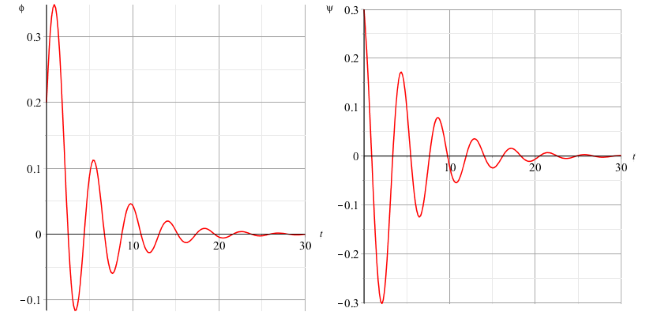
\includegraphics{pendulum}
	\caption{Результаты моделирования при управлении (\ref{1.46'})}
	\label{fig:pendulum_1}
\end{figure}
 
	
	\chapter{Управление движением двузвенного манипулятора}
	\section{Постановка задачи} \label{p21}
\paragraph{}
Рассмотрим математическую модель двухзвенного манипулятора. Манипулятор состоит из неподвижного основания и двух абсолютно жестких звеньев $G_1, G_2$. Элементы конструкции соединены между собой двумя идеальными цилиндрическими шарнирами $O_1,$ и $O_2$ таким образом, что оба звена могут совершать движения только в горизонтальной или вертикальной плоскости. Центр масс $C_1$ звена $G_1$ лежит на луче $O_1 O_2.$ Положение центра масс $C_2$ звена $G_2$ не совпадает с положением шарнира $O_2$.

 \begin{figure}[h]
 	\centering
 	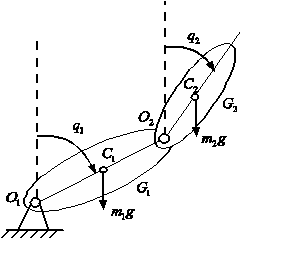
\includegraphics{manipulator}
 	\caption{Модель двузвенного манипулятора}
 	\label{fig:manip1}
 \end{figure}

Введем обозначения: $q_i (i=1, 2)$ --- углы поворотов звеньев манипулятора, показанные на рисунке; $l_i$ --- длина отрезка $O_i C_i;$ $l$ --- длина отрезка $O_1 O_2;$ $m_i$  ---  масса   $i$-го звена;   $I_i$ --- момент инерции  $i$-го звена относительно оси шарнира $O_i;$ $g$ --- ускорение свободного падения.

Выражение для кинетической энергии манипулятора имеет в таком случае следующий вид:
\begin{equation}
T = \frac12 ((I_1 + I_2 + m_2 l^2 + 2 m_2 l l_2 \cos q_2) \dot q_1^2 + (I_2 + m_2 l l_2 \cos q_2) \dot q_1 \dot q_2 + I_2 \dot q_2^2)
\end{equation}

Составим уравнения Лагранжа второго рода:

\begin{equation}
\begin{cases}
\displaystyle \frac{d}{dt} (\frac{\partial T}{\partial \dot q_1}) - \frac{\partial T}{\partial q_1} = M_1 + U_1, \\
\displaystyle \frac{d}{dt} (\frac{\partial T}{\partial \dot q_2}) - \frac{\partial T}{\partial q_2} = M_2 + U_2,
\end{cases}
\end{equation}

где $M_i$ --- момент, создаваемый силой тяжести в $i$-м шарнире. В случае манипулятора, совершающего движения в вертикальной плоскости, 
$$
\begin{array}{l}
M_1 = (m_1 l_1 + m_2 l) g \cos q_1, \\
M_2 = m_2 l_2 g \cos (q_1 + q_2),
\end{array}
$$
$U_i$ --- управление.

Из выражения для кинетической энергии $T$ находим уравнения движения

\begin{equation}
\begin{array}{l}
a_{11} \ddot q_1 + a_{12} \ddot q_2 - 2 m_2 l l_2 \sin q_2 \dot q_1 \dot q_2 - m_2 l l_2 \sin q_2 \dot q_2^2 = M_1 + U_1,\\ 
a_{12} \ddot q_1 + a_{22} \ddot q_2 + m_2 l l_2 \sin q_2 \dot q_1^2 = M_2 + U_2,\\
a_{11} (q_2) = m_2 l_1^2 + I_1 + I_2 + 2 m_2 l l_2 \cos q_2,\\
a_{12} (q_2)= I_2 + m_2 l l_2 \cos q_2, a_{22} = I_2
\end{array}
\end{equation}

\begin{equation}
\begin{array}{l}
	a_{11} \ddot q_1 + a_{12} \ddot q_2 - 2 m_2 l l_2 \sin q_2 \dot q_1 \dot q_2 - m_2 l l_2 \sin q_2 \dot q_2^2 = M_1 + U_1,\\ 
	a_{12} \ddot q_1 + a_{22} \ddot q_2 + m_2 l l_2 \sin q_2 \dot q_1^2 = M_2 + U_2,\\
	\dot x_1 = \sin(q_1(t)) - k * x_1(t), \\ 
	\dot x_2 = \sin(q_2(t)) - k * x_2(t), \\ 
	a_{11} (q_2) = m_2 l_1^2 + I_1 + I_2 + 2 m_2 l l_2 \cos q_2,\\
	a_{12} (q_2)= I_2 + m_2 l l_2 \cos q_2,\\ 
	a_{22} = I_2
\end{array}
\end{equation}

$U1 = -\mu_1 \sin(q_1(t)) - \frac{L}{k} \sin(q_1(t)) \cos(q_1(t)) (1 - e^{- k t}) + L x_1(t) \cos(q_1(t))$

$U2 = -\mu_2 \sin(q_2(t)) - \frac{L}{k} \sin(q_2(t)) \cos(q_2(t)) (1 - e^{- k t}) + L x_2(t) \cos(q_2(t))$

$q_1(0) = 0.5, \ \dot q_1(0) = -0.5, \ q_2(0) = 2.1, \ \dot q_2(0) = 0.3, \ x_1(0) = 0, \ x_2(0) = 0$

$$ I_1 = 3.33, \ I_2 = 3.33,  l = 1,  l_2 = 0.5,  m_2 = 10, \mu_1 = 5,  \mu_2 = 5, L = 1,  k = 1$$

Пусть $q=q(q_1, q_2)^{'}$ --– вектор обобщенных координат рассматриваемой механической системы и 
$$X = \{(q^0(t), \dot q^0(t)) : [t_0, + \infty) \to R^4, \|q^0(t)\| \le g_0, \|\dot q^0(t) \| \le g_1, \|\ddot q^0(t)\| \le g_2 \}$$

есть заданное множество программных движений манипулятора в виде ограниченных дважды непрерывно дифференцируемых функций $q=q^0(t)$ с ограниченными производными при $t \in [t_0, + \infty).$ Символом $\| \cdot \|$   обозначена евклидова норма вектора.

Пусть $(q^0(t), \dot q^0(t)) \in X$ --- какое-либо программное движение, реализуемое программным управлением $U = U^0(t).$ Таким образом, для обеспечения такого движения имеет место следующее управление
$$
\begin{array}{l}
U_1^0 (t) = a_{11} (q_2^0 (t)) \ddot q_1^0 (t) + a_{12} (q_2^0 (t)) \ddot q_2^0 (t) - 2 m_2 l l_2 \sin q_2^0 (t) \dot q_1^0 (t) \dot q_2^0 (t) - \\ 
- m_2 l l_2 \sin q_2^0 (t) - M_1^0 (t) \\
U_2^0 (t) = a_{12}^0 (t) \ddot q_1^0 (t) + I_2 \ddot q_2^0 (t) - M_2^0 (t) \\
\end{array}
$$
где $M_1^0(t) = M_2^0(t) = 0$ для случая манипулятора в горизонтальной плоскости
$$
\begin{array}{l}
M_1^0 (t) = (m_1 l_1 + m_2 l) g \cos q_1^0 (t), \\
M_2^0 (t) = m_2 l_2 g \cos (q_1^0 (t) + q_2^0 (t))
\end{array}
$$

в случае манипулятора, функционирующего в вертикальной плоскости.

Введем возмущения $x_k = q_k - q_k^0(t), \quad \dot x_k = \dot q_k - \dot q_k^0(t), \quad k = 1, 2$

Составим уравнения возмущенного движения в векторно-матричном виде:
\begin{equation}
A^{(1)}(t, x) \ddot x = {\dot x^{'} C^{(1)}(t, x) \dot x} + Q^{(1)}(t,x) + Q^{(2)}(t, x, \dot x) + U^{(1)}, \label{2.2'}
\end{equation}

$$A^{(1)}(t, x) =
\begin{pmatrix}
a_{11} (q_2^0 (t) + x_2) && a_{12} (q_2^0 (t) + x_2) \\
a_{12} (q_2^0 (t) + x_2) && I_2 \\
\end{pmatrix}$$

$$ C^{(1)}(t,x), \quad Q^{(1)}(t,x)=F(t,x)p(x), \quad Q^{(2)}(t,x,\dot x)=D(t,x)\dot x, $$

$$C_1^{(1)}(t, x) = m_2 l l_2 \sin (q_2^0 (t) + x_2)
\begin{pmatrix}
0 && 1\\
1 && 1\\
\end{pmatrix}$$

$$C_2^{(1)}(t, x) = - m_2 l l_2 \sin (q_2^0 (t) + x_2)
\begin{pmatrix}
1 && 0\\
0 && 0\\
\end{pmatrix}$$

$$ C^{(1)}(t, x) =
\begin{mpmatrix}
- m_2 l l_2 \sin(q_2^0(t) - q_1^0(t) + x_2 - x_1) && 0 \\
0 && m_2 l l_2 \sin(q_2^0(t) - q_1^0(t) + x_2 - x_1) \\
\end{mpmatrix}, $$

$$F(t, x) =
\begin{pmatrix}
f_{11}(t,x) && f_{12}(t,x) \\
f_{21}(t,x) && f_{22}(t,x)\\
\end{pmatrix},$$

$$p(x) =
\begin{pmatrix}
\sin(x_1/2) \\
\sin(x_2/2)\\
\end{pmatrix},$$

$$D(t, x) =
\begin{pmatrix}
d_{11} (t, x) && d_{12} (t, x) \\
d_{21} (t, x) && d_{22} (t, x) \\
\end{pmatrix},$$

$f_{11}(t,x) = 0 + \{ (- 2 m_1 l_1 - 2 m_2 l) g \sin (q_1^0 (t) + x_1 / 2) \}$

$f_{12}(t,x) = 4 m_2 g l l_2 \ddot q_1^0 (t) \sin (q_2^0 (t) + x_2 / 2) + 2 m_2 l l_2 \ddot q_2^0 (t) * \\ 
* \sin (q_2^0 (t) + x_2 / 2) + 4 m_2 l l_2 \cos (q_2(t) + x_2 / 2) \dot q_1^0 (t) \dot q_2^0 (t) + \\ 
+ 2 m_2 l l_2 \cos (q_2^0 (t) + x_2 / 2) (\dot q_2^0)^2$

$f_{21}(t,x) = 0 + \{ (-4 m_2 l_2 g \sin (q_1^0 (t) + q_2^0 (t) + x_1 /2 + x_2 / 2 \cos x_2 / 2)) \}$

$f_{22}(t,x) = 2 m_2 l l_2 \ddot q_2^0 (t) \sin (q_2^0 (t) + x_2 / 2) + 2 m_2 l l_2 \cos (q_2^0 (t) + x_2 /2) * \\ 
* (q_1^0 (t))^2 + \{ (-4 m_2 l_2 \sin (q_1^0 (t) + q_2^0 (t) + x_1 / 2 + x_2 /2) \cos x_1 /2) \}$

$$
\begin{array}{l}
d_{11}(t, x) = 2 m_2 l l_2 \sin(q_2^0 (t + x_1) \dot q_2^0 (t)) \\
d_{12}(t, x) = 2 m_2 l l_2 \sin(q_2^0 (t + x_1) \dot q_1^0 (t)) + 2 m_2 l l_2 \sin(q_1^0 (t) + x_2) \dot q_2^0 (t) \\
d_{21}(t, x) = - 2 m_2 l l_2 \sin (q_2^0 (t) + x_2) \dot q_1^0 (t) \\
d_{22}(t, x) = 0
\end{array}
$$

где слагаемые, заключенные в фигурные скобки, добавляются в случае вертикального манипулятора.

$$ U^{(1)} = U - U^{0}(t) $$

В главе рассматривается задача построения управляющего воздействия $$ U^{(1)} = U^{(1)}(t, x, \dot x), \quad U^{(1)} (t, 0, 0) \equiv 0 $$, при котором бы невозмущенное движение $\dot x = x = 0$  системы (2.2) было бы равномерно асимптотически устойчиво, или, иными словами, управление $$U = U^0(t) + U^{(1)}(t, q-q^0(t), \dot q - \dot q^0(t))$$

обеспечивало бы стабилизацию программного движения $(q^0(t), \dot q^0(t)) \in X$  системы (2.1).
	\section{Стабилизация положения равновесия модельного уравнения} \label{p22}
	\section{Об управлении двузвенным манипулятором с приводом} \label{p23}

Рассмотрим решение задачи стабилизации в области 
$$G = {(x, \dot x) \in R^4 : \|x\|<\varepsilon, \quad \|\dot x\|<\varepsilon, \quad \varepsilon=const>0}$$
с помощью непрерывного управления вида
$$U^{(1)}(x, \dot x) = B(\dot x + p(x))$$ \label{2.3'}     
где $B \in R^{2 \times 2}$ есть матрица коэффициентов усиления сигналов, подлежащая определению.
Возьмем для системы (2.2) вектор-функцию Ляпунова $V = (V^1, V^2)^{'}$  с коэффициентами вида $$V^1 = \|p(x)\|, \quad V^2 = \sqrt{(\dot x + p(x))^{'} A^{(1)}(t, x)(\dot x + p(x)).}$$
Вычисляя производную по времени вектор-функции Ляпунова $V$ в силу системы (2.1), получим следующие оценки:
$$
\begin{array}{l}
\dot V^1 \le -mu_1 V^1 + \frac{m_1}{\lambda_1},\\
\dot V^2 \le m_2 V^1 - \mu_2 V^2 + m_3 (V^1)^2 + m_4 (V^2)^2 + m_5 V^1 V^2, 
\end{array}
$$

где положительные постоянные $\mu_1, \mu_2, \lambda_1, m_i (i=1,2,...,5)$ определяются из следующих условий:
$$
\begin{array}{l}
\displaystyle \lambda_1^2 = \frac{I_1 + m_2 l_1^2 + I_2 - \sqrt{(I_1 + m_2 l_1^2 - I_2)^2} + 4(m_2 l_1 l_{g_2})^2}{2}\\
\displaystyle \lambda_2^2 = \frac{I_1 + m_2 l_1^2 + I_2 + \sqrt{(I_1 + m_2 l_1^2 - I_2)^2} + 4(m_2 l_1 l_{g_2})^2}{2}\\
\displaystyle \mu_1 =\frac12 \cos(\frac{\varepsilon}{2}), \quad m_1 = \frac12,\\
\displaystyle m_2 = \max \frac{\lambda_2^2 + 2 \sqrt{\lambda_{max} [(D-F)^{'} (D-F)]}}{2 \lambda_1},\\
\displaystyle m_3 = \frac{m_2 l_1 l_{g_2}}{\lambda_1}, \quad m_4 = \frac{2 m_2 l_1 l_{g_2}}{\lambda_1}, \quad m_5 = \frac{3 m_2 l_1 l_{g_2}}{\lambda_1},\\
\displaystyle \mu_2 = \frac{-\lambda_2^2 - 4 g_1 m_2 l_q l_{g_2} - \lambda_{max} (B + B^{'})}{2 \lambda_2}
\end{array}
$$

Здесь $\lambda_{max}$ есть максимальное собственное значение соответствующей матрицы. 
Тогда для системы (2.1) можно построить следующую систему сравнения:

\begin{equation}\label{2.4'}
\dot u^1 = - \mu_1 u^1 + \frac{m_1}{\lambda_1} u^2, \quad \dot u^2 = m_2 u^1 - \mu_2 u^2 + m_3 (u^1)^2 + m_4(u^2)^2 + m_5 u^1 u^2
\end{equation}

Согласно теореме сравнения об асимптотической устойчивости [5] из свойства асимптотической устойчивости нулевого решения системы сравнения (2.4) следует свойство равномерной асимптотической устойчивости нулевого решения системы (2.2). Получим условие асимптотической устойчивости нулевого решения системы (2.4) с областью притяжения $ {(u^1, u^2) \in R^2 : 0 \le u^1 \le \delta_1 = const>0, 0 \le u^2 \le \delta_2 = const>0} $ . Пусть найдется такое число $\gamma>0$, что выполняются соотношения:

\begin{equation}\label{2.10'}
\gamma = \frac{\delta_2 m_1}{\delta_1 \lambda_1 \mu_1}, \quad \mu_2 > \frac{m_1}{\gamma \lambda_1 \mu_1} (m_2 + \delta_1 m_3) + m_4 \delta_2 + m_5 \delta_1
\end{equation}

Тогда можно показать, что функция $\widetilde{u}(t) = \max{(u^1(t), \delta_1 u^2(t)/ \delta_2)}$ будет монотонно стремиться к нулю при $t \to \infty$, и, значит, нулевое решение системы сравнения (2.4) будет асимптотически устойчиво.
При невозможности практической реализации программного управления стабилизацию программного движения можно осуществить при помощи разрывного управления вида

\begin{equation} \label{2.11'}
U^{(1)}(x, \dot x) = B \ sign(\dot x + p(x))
\end{equation}

Численное моделирование движения манипулятора при действии управлений (2.3) и (2.6) проводилось при следующих значениях параметров манипулятора и программной траектории:
$$
\begin{array}{l}
 m_1 = 0,5 \quad \text{кг}, \quad m_2 = 0,3 \text{кг}, \quad l_1 = 0,5 \text{м}, \quad l_2 = 0,5 \text{м }, \\ l_{g_1} = 0,25 \text{ м}, \quad l_{g_2} = 0,3 м, \quad I_1 = 0,01 \text{ кг} \cdot \text{м\textsuperscript{2}}, \quad I_2 = 0,006 \text{ кг} \cdot \text{м\textsuperscript{2}},\\
 \quad q_1^0(t) = \sin(0,5t), \quad q_1^0(t) = \cos(0,5t) + \pi/2
\end{array}
$$

На рисунках 2 и 3 представлены результаты моделирования при управлениях (2.3) и (2.6) соответственно. 

\begin{figure}[h]
	\centering
	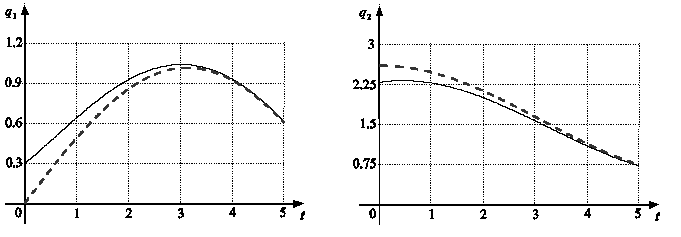
\includegraphics{model1}
	\caption{Результаты моделирования при управлении (2.3)}
	\label{fig:manip2}
\end{figure}

\begin{figure}[h]
	\centering
	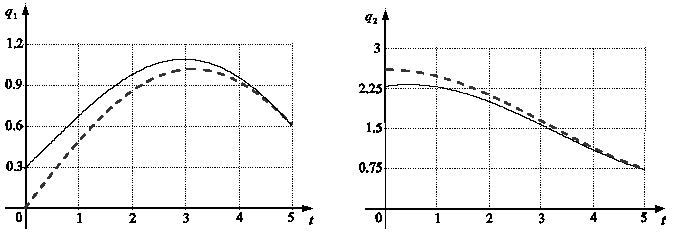
\includegraphics{model2}
	\caption{Результаты моделирования при управлении (2.6)}
	\label{fig:manip3}
\end{figure} 
	\section{Об управлении двузвенным манипулятором с приводом} \label{p24}

Рассмотрим манипулятор, моделируемый в виде механической системы, состоящей из неподвижного основания $G_0$ и двух абсолютно жестких звеньев $G_1, G_2$. Элементы конструкции соединены между собой двумя цилиндрическими шарнирами $O_1, O_2$ таким образом, что оба звена могут совершать движения только в горизонтальной плоскости под действием приводов, приложенных в этих шарнирах.

Будем считать, что приводы управляются некоторыми воздействиями $L_{i}$ в соответствии с уравнениями 

\begin{equation} \label{2.14'}
\frac{d M_i}{dt} = L_{i}
\end{equation}

Рассматривается задача построения структуры обратной связи в виде зависимости $L_{i} = L_{i} (t, q, \dot q, M)$ таким образом, чтобы каждое программное движение системы $(q_1 (t), q_2 (t))$ являлось бы асимптотически устойчивым. 

Продемонстрируем решение этой задачи для случая положения равновесия системы

\begin{equation} \label{2.15'}
\dot q_1 = \dot q_2 = 0, \quad q_1 = q_2 = 0, \quad M_1 = M_2 = 0
\end{equation}

Покажем, что такая задача решается управлением приводами со следующим видом обратной связи

\begin{equation}  \label{2.16'}
L_1 = - M_1 - k_1 (\dot q_1 + \beta_1 \sin \frac{q_1}{4}), \quad L_2 = - M_2 - k_2 (\dot q_2 + \beta_2 \sin \frac{q_2}{4})
\end{equation}

где $k_1, k_2, \beta_1, \beta_2 > 0$ есть некоторые постоянные, определяемые из условия стабилизации положения равновесия (\ref{2.15'}).

Для нахождения этих условий применим метод векторых функций Ляпунова \cite{matrosov01}, в соотвтетствии с методикой их построения, представленной в \cite{andr111}.

Векторную функцию Ляпунова возьмем в виде
$$
\begin{array}{l}
V_1 = \sqrt{c_1 \sin^2 \frac{q_1}{4} + c_2 \sin^2 \frac{q_2}{4}}, \quad c_1, c_2 > 0\\
V_2 = \sqrt{a_{11} (\dot q_1 + \beta_1 \sin \frac{q_1}{4})^2 + 2 a_{12} (\dot q_1 + \beta_1 \sin \frac{q_1}{4}) (\dot q_2 + \beta_2 \sin \frac{q_2}{4}) + a_{22} (\dot q_2 + \beta_2 \sin \frac{q_2}{4})^2}\\
V_3 = \sqrt{p_{11} (M_1 + k_1 (\dot q_1 + \beta_1 \sin \frac{q_1}{4})^2) + 2 p_{12} (M_1 + k_1 (\dot q_1 + \beta_1 \sin \frac{q_1}{4})) (M_2 + k_2 (\dot q_2 + \beta_2 \sin \frac{q_2}{4})) + p_{22} (M_1 + k_1 (\dot q_2 + \beta_2 \sin \frac{q_2}{4}))^2}\\
a_{11} > 0, a_{11} a_{22} > 0, p_{11} > 0, p_{11} p_{22} - p_{12}^2 > 0
\end{array}
$$ 

Для производной функции $V_1$ в силу (\ref{2.12'}), (\ref{2.13'}), (\ref{2.15'}) 
при $\| q_1 \| \le \Pi, \quad \| q_2 \| \le \Pi$ находим оценку 
$$
\begin{array}{c}
\dot V_1 = \frac{1}{4 V_1} (c_1 \sin \frac{q_1}{4} \cos \frac{q_1}{4} - \dot q_1 + c_2 \sin \frac{q_2}{4} \cos \frac{q_1}{4} \dot q_2) =\\
= \frac{1}{4 V_1} (c_1 \sin \frac{q_1}{4} \cos \frac{q_1}{4} (\dot q_1 + \beta_1 \sin \frac{q_1}{4} - \beta_2 \sin \frac{q_1}{4}) +\\
+ c_2 \sin \frac{q_2}{4} \cos \frac{q_2}{4} (\dot q_2 + \beta_2 \sin \frac{q_2}{4} - \beta_2 \sin \frac{q_2}{4})) \le\\
\le \frac{1}{4 V_1} (\sqrt{c_1 \sin^2 \frac{q_1}{4} + c_2 \sin^2 \frac{q_2}{4}} \sqrt{c_1 (\dot q_1 + \beta_1 \sin \frac{q_1}{4})^2 +\\
+ c_2 (\dot q_2 + \beta_2 \sin \frac{q_2}{4})^2} - \frac{\sqrt{2}}{2} (c_1 \beta_1 \sin^2 \frac{q_1}{4} c_2 \beta_2 \sin^2 \frac{q_2}{4})) \le\\
\le - \alpha_1 V_1 + \alpha_2 V_2, \alpha_1 = \frac{\sqrt{2}}{8} min(\sqrt{c_1} \beta_1, \sqrt{c_2}, \beta_2), \alpha_2 = \frac{1}{4} \sqrt{\lambda_{AC}^{max}}
\end{array}
$$

где $\lambda_{AC}^{max}$ - наибольшее характеристическое значение матрицы $c = diag(c_1, c_2)$ на пучке матриц $A = A(q).$

Для производной от функции $V_2$ в силу (\ref{2.12'}), (\ref{2.13'}), (\ref{2.15'}) имеем более сложную оценку.
$$
\begin{array}{c}
\dot V_2 = \frac{1}{V_2} ((\dot q_1 + \beta_1 \sin \frac{q_1}{4}) ((M_1 + k_1 (\dot q_1 + \beta_1 \sin \frac{q_1}{4})) -\\
- k_1 (\dot q_1 + \beta_1 \sin \frac{q_1}{4}) + \frac{1}{4} a_{11} \beta_2 \cos \frac{q_1}{4} (\dot q_1 + \beta_1 \sin \frac{q_1}{4}) - \frac{1}{4} a_{11} \beta_1^2 \cos \frac{q_1}{4} \sin \frac{q_1}{4}) +\\
+ 2 m_2 l_1 l_2 \sin q_2 (\dot q_2 + \beta_2 \sin \frac{q_2}{4} - \beta_2 \sin \frac{q_2}{4})^2) +\\
+ (\dot q_2 + \beta_2 \sin \frac{q_2}{4}) (M_2 + k_2 (\dot q_2 + \beta_2 \sin \frac{q_2}{4}) -\\
- k_2 (\dot q_2 + \beta_2 \sin \frac{q_1}{4}) + \frac{1}{4} a_{12} \beta_2 \cos \frac{q_2}{4} (\dot q_2 + \beta_2 \sin \frac{q_2}{4}) -\\
- \frac{1}{4} a_{22} \beta_2^2 \cos \frac{q_2}{4} \sin \frac{q_2}{4} -\\
- m_2 l_1 l_2 \sin q_2 (\dot q_1 + \beta_1 \sin \frac{q_1}{4} - \beta_1 \sin \frac{q_1}{4})^2) \le\\
\le \gamma_1 V_1 - \gamma_2 V_2 + \gamma_3 V_3 + \mu_{21} V_1^2 + \mu_{22} V_2^2 + \mu_{23} V_3^2, \gamma_1 =\\
= \frac{p_{max}}{\lambda_{min}}, \gamma_2 = \frac{1}{\lambda_{min}}, \gamma_3 = \frac{1}{4} a_{max} \beta_{max}
\end{array}
$$

где $\mu_{21}, \mu_{22}, \mu_{23}$ зависят от параметров системы и управления.

Для производной функции $V_3$ более сложными вычислениями получим оценку

$\dot V_3 \le V_1 + V_2 - V_3 + \mu_{31} V_1^2 + \mu_{32} V_2^2 + \mu_{33} V_3^2$

$\nu_1 = \frac{2}{\sqrt{\lambda_{min}}} (a_{11} + \| a_{12} \|) \beta_1, \nu_2 = \frac{2}{\sqrt{\lambda_{min}}} (\| a_{12} \| + a_{22}) \beta_1$

$\nu_3 = k - 2 ((a_{11} + \| a_{12} \|) \beta_1 + (\| a_{12} \| + a_{22}) \beta_2), k = \min (k_1, k_2), $

где $\mu_{3i} > 0$ - некоторые коэффициенты, выражаемые через параметры $k_i, \beta_i$.

Стабилизация движения (\ref{2.14'}) согласно теореме об асимптотической устойчивости из \cite{matrosov01} в самой общей постановке может определяться системой

$\dot y_1 = - \alpha_1 y_1 + \alpha_2 y_2$

$\dot y_2 = \gamma_1 y_1 - \gamma_2 y_2 + \gamma_3 y_3 + \gamma_{31} y_1^2 + \mu_{22} y_2^2 + \mu_{33} y_3^2$

$\dot y_3 = \nu_1 y_1 + \nu_2 y_2 - \nu_3 y_3 + \mu_{31} y_1^2 + \mu_{32} y_2^2 + \mu_{33} y_3^2$

При малых возмущениях стабилизация находится из асимптотической устойчивости линейной системы

$\dot y_1 = - \alpha_1 y_1 + \alpha_2 y_2, \dot y_2 = \gamma_1 y_1 - \gamma_2 y_2 + \gamma_3 y_3, \dot y_3 = \nu_1 y_1 + \nu_2 y_2 - \nu_3 y_3$

Ниже представлены результаты численного моделирования процесса стабилизации положения при следующих численных значениях $\mu_1 = 1, k_1 = 5, \beta_1 = 6, \mu_2 = 1, k_2 = 4, \beta_2 = 7, q_{10} = 0,5, q_2 = 0,8, \dot q_{10} = 0,6, \dot q_{20} = 0,8, M_{10} = 0,9, M_{20} = 0,7, \mu_{20} = 0,7, l_1 = 1 м, l_{g_2} = 0,5 м, I_1 = I_2 = 3,33 кг м 3, m_2 = 10 кг$ 

\begin{figure}[h]
	\centering
	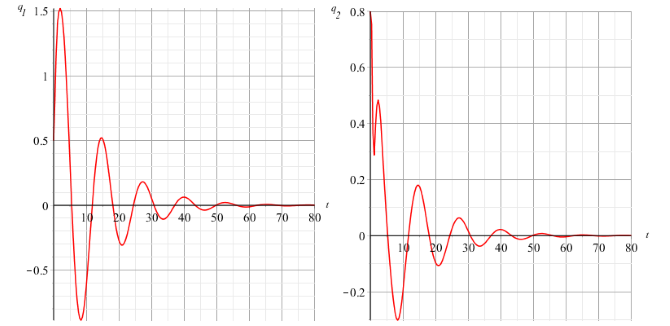
\includegraphics{with_gears}
	\caption{Результаты моделирования при управлении (2.16)}
	\label{fig:manip22}
\end{figure} 
	
	\chapter{Управление движением трехзвенного манипулятора (без привода и с приводом)}
	
\section{Стабилизация программных движений голономной механической системы } \label{p31}
\paragraph{}
 Рассмотрим математическую модель трехзвенного манипулятора, состоящую из трех абсолютно жестких звеньев $G_1, G_2, G_3$, представляющих собой однородные стержни. Манипулятор установлен на неподвижном основании, на которое опирается звено $G_1$. Звено $G_1$ таким образом, может совершать только вращения вокруг вертикальной оси. Звенья соединены между собой двумя идеальными цилиндрическими шарнирами $O_1$, и $O_2$ таким образом, что звенья $G_2$ и $G_3$ могут совершать движения только в вертикальной плоскости. Центр масс $C_1$ звена $G_1$ лежит на луче  $O_1 O_2$. Положение центра масс $C_2$ звена $G_2$ не совпадает с положением шарнира $O_2$. На конце звена $G_3$ находится груз, перемещаемый манипулятором.
 
 Введем обозначения: $q_i (i=1, 2, 3)$ --- углы поворотов звеньев манипулятора; $Q_i (i = 1, 2, 3)$ ---  управляющие моменты относительно осей соответствующих звеньев; $l_i$  ---  длина   $i$-го звена;   $m_i$ --- масса  $i$-го звена;    $m_0$ ---  масса перемещаемого груза;  $m_{30} = m_0 + m_3$; $J_{01}$  ---  момент инерции первого звена относительно оси вращения; $r_2$ и $r_3$ --- соответственно расстояния от центров тяжести второго и третьего звеньев с перемещаемым грузом относительно осей соответствующих звеньев; $g$ --- ускорение свободного падения.
 Уравнения движения манипулятора имеют вид:
 
 \begin{equation}
 \begin{cases}
 (J_{01} + m_2 r_2^2 \sin^2 q_2 + m_{30} (l_2 \sin q_2 + r_3 \sin q_3)^2) \ddot q_1 + \\ + 2 (m_2 r_2^2 \sin q_2 \cos q_2 + m_{30} (l_2 \sin q_2 + r_3 \sin q_3) l_2 \cos q_2) \dot q_1 \dot q_2 + \\ + 2 m_{30} (l_2 \sin q_2 + r_3 \sin q_3) r_3 \cos q_3 \dot q_1 \dot q_3 = Q_1,
 \\
 (m_2 r_2^2 + m_3 l_2^2) \ddot q_2 + \frac12 m_{30} l_2 r_3 \cos(q_2 - q_3) \ddot q_3 + \frac12 m_{30} l_2 r_3 \sin (q_2 - q_3) \dot q_3^2 - \\ - (m_{30} (l_2 \sin q_2 + r_3 \sin q_3) l_2 + m_2 r_2^2 \sin q_2) \cos q_2 \dot q_1^2 + (m_2 r_2 + m_{30} l_2) g \sin q_2 = Q_2,
 \\
 \frac12 m_{30} l_2 r_3 \cos(q_2 - q_3) \ddot q_2 + m_{30} r_3^2 \ddot q_3 - \frac12 m_{30} l_2 r_3 \sin (q_2 - q_3) \dot q_2^2 - \\ - m_{30} (l_2 \sin q_2 + r_3 \sin q_3) r_3 \cos q_3 \dot q_1^2 + m_{30} g r_3 \sin q_3 = Q_3.
 \end{cases}
 \end{equation}
 
 \begin{figure}[h]
 	\centering
 	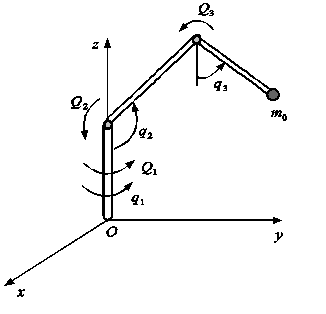
\includegraphics{3chain}
 	\caption{Модель трехзвенного манипулятора}
 	\label{fig:manip1}
 \end{figure}
 
 Пусть $q=(q_1, q_2, q_3)$ --- вектор обобщенных координат представленной выше системы. Таким образом, уравнения движения можно представить в следующей векторно-матричной форме: $A(q) \ddot q + C(q, \dot q) \dot q + K \dot q = Q$ где 
 
 \vspace{5mm}
 
 $$A(q) =
 \begin{pmatrix}
 a_{11} && 0 && 0  \\
 0  && a_{22} && a_{23} \\
 0 && a_{32} &&  a_{33}\\
 \end{pmatrix}$$
 
 \vspace{5mm}
 
 Элеменыт матрицы инерции $A(q):$
 
 $$a_{11} = J_{01} + m_2 r_2^2 \sin^2 q_2 + m_{30} (l_2 \sin q_2 + r_3 \sin q_3)^2$$
 $$a_{22} = m_2 r_2^2 + m_3 l_2^2$$
 $$a_{23} = \frac12 m_{30} l_2 r_3 \cos(q_2 - q_3)$$
 $$a_{32} = a_{23}$$
 $$a_{33} = m_{30} r_3^2$$
 
 $$C(q, \dot q)= 
 \begin{pmatrix}
 c_{11} && 0 && c_{13} \\
 c_{21} && 0 && 0 \\
 c_{31} && c_{32} && 0\\
 \end{pmatrix}$$
 
 Элементы матрицы $C(q, \dot q):$
 
 $$c_{11} = 2 (m_2 r_2^2 \sin q_2 \cos q_2 + m_{30} (l_2 \sin q_2 + r_3 \sin q_3) l_2 \cos q_2) \dot q_2$$
 $$c_{13} = 2 m_{30} (l_2 \sin q_2 + r_3 \sin q_3) r_3 \cos q_3 \dot q_3$$
 $$c_{21} = - (m_{30} (l_2 \sin q_2 + r_3 \sin q_3) l_2 + m_2 r_2^2 \sin q_2) \cos q_2 \dot q_1$$
 $$c_{31} = - m_{30} (l_2 \sin q_2 + r_3 \sin q_3) r_3 \cos q_3 \dot q_1$$
 $$c_{32} = - \frac12 m_{30} l_2 r_3 \sin (q_2 - q_3) \dot q_2$$
 
 \vspace{5mm}
 
 $A(q)$ --- положительно определенная матрица инерции системы.
 
 \section{Построение управления}%
 \markright{\thechapter.\thesection.\hspace{1em}Построение управления}{}
 \label{sec2.3}
 Пусть  $q = (q_1, q_2, q_3)^{'}$ --- вектор обобщенных координат рассматриваемой механической системы и $X = {q^0(t):[t_0, + \infty) \to R^3, \| q^0(t) \| \le q_0, \| \dot q^0 \| \le g_1,\| q^0(t) \| \le q_0, \| \ddot q^0 \| \le g_2}$ есть заданное множество программных движений манипулятора в виде ограниченных дважды непрерывно дифференцируемых функций $q = q^0(t)$ с ограниченными производными при $t \in [t_0, + \infty)$.  Символом   $\| \cdot \|$ обозначена евклидова норма вектора. Уравнения движения (3.1) можно представить в следующей векторно-матричной форме: 
 
 \begin{equation}
 A(q) \ddot q + C(q, \dot q) \dot q + K \dot q = Q,     
 \end{equation}

 где $A(q)$ --- положительно определенная матрица инерции системы, $C(q, \dot q) = \sum_{i = 1}^{3} \dot q_i C_{(i)} (q),$ , $j,k$-ый элемент $c_{(i)jk} (q)$ матрицы $C_{(i)}(q)$  определяется в виде $c_{(i)jk} (q) = \frac12 (\frac{\partial a_{ij}}{\partial q_k} + \frac{\partial a_{ij}}{\partial q_i} - \frac{\partial a_{ij}}{\partial q_j} )$;
 $K$ --- матрица коэффициентов моментов сил вязкого трения, действующих в системе.
 Система (3.2) имеет следующее свойство: матрица $\dot A(q(t)) - 2 C(q(t), \dot q(t))$  является  кососимметричной.
 Пусть $q^0(t) \in X$ --- какое-либо программное движение системы (3.2), реализуемое программным управлением $Q = Q^{(0)}(t)$, т.е. имеет место тождество $A(q^0(t)) \ddot q^0(t) + C(q^0(t), \dot q^0(t)) \dot q^0(t) + K \dot q^0(t) \equiv Q^{(0)}(t)$.
 Введем возмущения $x = q - q^0(t)$ и составим уравнения возмущенного движения в векторно-матричном виде:
 \begin{equation}
 A^{(1)}(t, x) \ddot x + C^{(1)}(t, x, \dot x) \dot x + K \dot x = Q^{(1)}(t, x, \dot x) + Q^{(2)}(t, x, \dot x),
 \end{equation} 
 где $A^{(1)}(t, x) = A(x + q^0(t))$, $C^{(1)}(t, x, \dot x) = C(x + q^0(t)$, $\dot x + \dot q^0(t))$, $Q^{(1)}(t, x, \dot x) = Q - Q^{(0)}(t)$, $Q^{(2)}(t, x, \dot x) = (A^{(1)}(t, 0) - A^{(1)}(t, x)) \ddot q^0(t) + (C^{(1)}(t, 0, 0) - C^{(1)}(t, x, \dot x)) \dot q^0(t)$.
 Рассмотрим задачу построения управляющего воздействия $Q^{(1)}(t, x, \dot x)$, при котором невозмущенное движение $\dot x = x = 0$ системы (3.3) было бы равномерно асимптотически устойчиво, или, иначе, управление $Q = Q^{(1)}(t, q-q^{(0)}(t), \dot q - \dot q^{(0)}) + Q^{(0)}(t)$ обеспечивало бы стабилизацию программного движения   системы (3.2).
 
  \section{Синтез управления в задаче стабилизации программного движения манипулятора}% 
 Рассмотрим решение задачи стабилизации в области $G = {(x, \dot x) \in R^6 : \|x\| < \epsilon, \|\dot x \| < \epsilon, \epsilon = const>0}$
 с помощью непрерывного управления вида
 
 \begin{equation*}
  Q^{(1)} (x, \dot ) = B(\dot x + p(x)),
 \end{equation*}
 
 где $B \in R^{3 \times 3}$ есть матрица коэффициентов усиления сигналов, подлежащая определению; $p(x)$ --- непрерывно дифференцируемая вектор-функция, такая, что $\| p(x) \| \ge p_0(x) > 0, p_0(0) = 0$.
 Возьмем для системы (3.3) вектор-функцию Ляпунова $V = (V^1, V^2)^{'}$ с коэффициентами вида $V^1 = \|p(x)\|, V^2 = \sqrt{(\dot x + p(x))^{'} A^{(1)} (t, x) (\dot x + p(x))}$.
 
 Вычисляя производные по времени от квадратов компонент вектор-функции Ляпунова  в силу системы (3.3), получим 
 \begin{equation*}
 \frac{d}{dt} (V^1(x))^2 = 2 V^1 \dot V^1 = 2 p^{'} \dot p = 2 p^{'} \frac{\partial p }{\partial x} \dot x = -2 p^{'} \frac{\partial p }{\partial x} p + 2 p^{'} \frac{\partial p }{\partial x}(\dot x + p),
 \end{equation*}
 
 \begin{equation*}
  \frac{d}{dt} (V^2(x))^2 = 2 V^2 \dot V^2 = 2(\ddot x + \dot p)^{'} A^{(1)} (\dot x + p) + (\dot x + p)^{'} \dot A^{(1)} (\dot x + p) = 2(- C^{(1)}(t, x, \dot x) \dot x - R \dot x + Q^{(1)}(x, \dot x) + Q^{(2)}(t, x, \dot x))^{'} (\dot x + p) + 2 \dot p^{'} A^{(1)} (\dot x + p) + (\dot x + p)^{'} \dot A^{(1)} (\dot x + p).
 \end{equation*}
 
 Отсюда получим следующие оценки:
 $\dot V^1 \le - \mu_1 V^1 + \frac{m_1}{\lambda(t, x)} V^2, \dot V^2 \le \frac{m_2}{\lambda(t, x)} V^1 - \frac{\mu_2}{\lambda^2(t,x)}$,
 где положительные постоянные $\mu_2, \mu_2, m_1, m_2$  и функция $\lambda(t,x)$  определяются из следующих условий:
 \begin{equation}
 p^{'} \frac{\partial p}{\partial x} p \ge \mu_1 \|p\|^2, \|\frac{\partial p}{\partial x}\| \le m_1, \lambda(t, x) \| \dot x + p \| = V^2,
 \end{equation}
 
 \begin{equation}
 \| Q^{(2)} (t, x, \dot x) \le (m_2 - \| C^{(1)}(t, x, \dot x) + K - A^{(1)}(t, x) \frac{\partial p}{\partial x}\|) \|p\|
 \end{equation}

\begin{equation}
 \lambda_{max} (B + B^{'} - K - K^{'} + A^{(1)}(t, x) \frac{\partial p}{\partial x} + (\frac{\partial p}{\partial x})^{'} A^{(1)}(t, x)) \le -2 \mu_2
\end{equation}
 
 Здесь $\lambda_max()$ есть максимальное собственное значение соответствующей матрицы. 
 Тогда для системы (3.3) можно построить следующую систему сравнения:
 
 \begin{equation}
 \dot u^1 = - \mu_1 u^1 + \frac{m_1}{\lambda(t,x)} u^2, \dot u^2 = \frac{m_2}{\lambda(t, x)} u^1 - \frac{\mu_2}{\lambda^2(t, x)} u^2. 
 \end{equation}
 
 Согласно теореме сравнения об экспоненциальной устойчивости [5] из свойства экспоненциальной устойчивости нулевого решения системы сравнения (3.5) следует аналогичное свойство нулевого решения системы (3.3).  Можно показать, что нулевое решение системы сравнения (3.5) будет экспоненциально устойчиво при следующем условии
 $4 \mu_1 \mu_2 > (m_1 / k + m_2 k)^2, k = const>0$.
 Численное моделирование движения манипулятора при действии управления (3.4) проводилось при следующих значениях параметров манипулятора и программной траектории
 
\begin{equation*}
 m_2=15 \text{ кг}, m_3=2,5 \text{ кг}, m_0 = 2 \text{ кг}, l_2 = 1 \text{ м}, r_2=0,5 \text{ м}, r_3 = 0,5 \text{ м}, J_{01} = 0,1 \text{ кг} \cdot \text{м\textsuperscript{2}}, q_1^0(t) = 0,2t, q_2^0(t) = 1,5 + 0,5 sin t, q_3^0(t) = 0,5 sin(0,5 t).
\end{equation*}
 
 На рисунках 2–4 представлены результаты моделирования. Пунктирной линией обозначены  составляющие программного движения, а сплошной – реального движения системы.
 
 
  \begin{figure}[h]
  	\centering
  	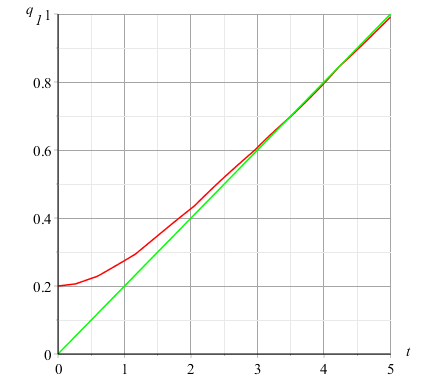
\includegraphics{pic1}
  	\caption{Зависимость угла поворота первого звена от времени при управлении (3.4) }
  	\label{fig:manip2}
  \end{figure}
  
  \begin{figure}[h]
    	\centering
    	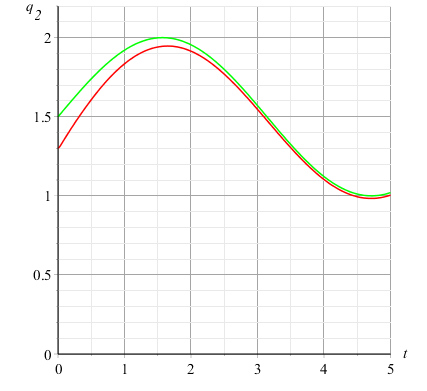
\includegraphics{pic2}
    	\caption{Зависимость угла поворота второго звена от времени при управлении (3.4)  }
    	\label{fig:manip2}
    \end{figure}
    
      \begin{figure}[h]
      	\centering
      	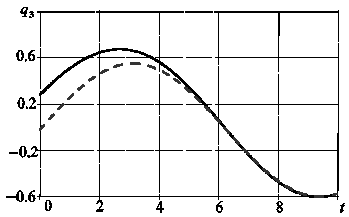
\includegraphics{pic3}
      	\caption{Зависимость угла поворота третьего звена от времени при управлении (3.4) }
      	\label{fig:manip2}
      \end{figure}
	\section{Моделирование управляемого движения  двузвенного манипулятора на подвижном основании} \label{p32}
	\section{Моделирование управляемого движения  двузвенного манипулятора на подвижном основании} \label{p33}

Здесь будет третий параграф третьей главы.
 
	
	{\centerline{ {\sc ЗАКЛЮЧЕНИЕ }} \label{postfix}
\paragraph{}
В представленной диссертационной работе разработаны новые методы стабилизации нелинейных управляемых систем, в частности многозвенных манипуляторов. Представлены новые методы исследования устойчивости.

Ниже представлены основные результаты работы.

\begin{enumerate}
	\item{Развитие метода векторных функций Ляпунова для исследования устойчивости нелинейных систем.}
	\item{Полученные результаты являются развитием соответствующих теорем из работ. Эффективность новой методики в исследовании и стабилизации представлена на примере решения задач стабилизации двух- и трехзвенных манипуляторов.}
	\item{Представлены модели двух- и трехзвенных манипуляторов, модель перевернутого маятника}
	\item{Разработана компьютерная модель движения трехзвенного манипулятора на неподвижном основании. Программный комплекс разработан на языке Java с использованием фреймворка JavaFX. Приложение является кроссплатформенным, позволяет задавать законы управления в аналитическом виде.}
\end{enumerate}

Основные результаты работы опубликованы в работах, в том числе, в статьях из списка ВАК. Получен патент РФ на программу для ЭВМ на программу моделирования движения трехзвенного манипулятора.

	
	\begin{thebibliography}{10} \label{bibl}
	\bibitem{abdullin00}
	{\it Абдуллин, Р. З.} Метод сравнения в устойчивости нелинейных разностных уравнений с импульсными воздействиями
	/ Р. З. Абдуллин // Автоматика и телемеханика.— 2000.— № 11.— С. 44-56. 	
	
	\bibitem{ajz747}
	{\it Айзерман, М.В} Основы теории разрывных систем I / М. А. Айзерман, Е. С. Пятницкий
	// Автоматика и телемеханика.— 1974.— № 7-8.— С. 33–47. С. 39–61.
	
	\bibitem{aleksandrov00}
	{\it Александров, В. В.} Оптимизация динамики управляемых систем / В. В. Александров, В. Г. Болтянский,
	С. С. Лемак и др.— М.: МГУ, 2000.— 303 с.
	
	\bibitem{ananev014}
	{\it Ананьевский, И. М.} Управление реономными механическими системами с неизвестными параметрами /
	И. М. Ананьевский // Докл. РАН.— 2001.— Т. 337, № 4.— С. 459–463.
	
	\bibitem{ananev012}
	{\it Ананьевский, И. М.} Два подхода к управлению механической системой с неизвестными параметрами /
	И. М. Ананьевский // Изв. РАН. Теор. и сист. упр.— 2001.— № 2.— С. 39–47.
	
	\bibitem{anap80}
	{\it Анапольский, Л. Ю.} Метод сравнения в динамике дискретных систем /
	Л. Ю. Анапольский; ред. В. М. Матросов, Л. Ю. Анапольский // Вектор-функции Ляпунова и их построение.— Новосибирск: Наука, 1980.— С. 92–128.
	
	\bibitem{andr15}
	{\it Андреев, А. С.} Об управлении движением колесного мобильного робота /
	А. С. Андреев, О. А. Перегудова // ПММ.— 2015.— Т. 79.— № 4.— С. 451–462.
	
	\bibitem{andr971}
	{\it Андреев, А. С.} О стабилизации управляемых систем с гарантированной оценкой качества управления /
	А. С. Андреев, С. П. Безгласный // ПММ.— 1997.— Т. 61.— № 1.— С. 44–51.
	
	\bibitem{andr124}
	{\it Андреев, А. С.} Метод векторной функции Ляпунова в задаче об управлении систем
	с мгновенной обратной связью / А. С. Андреев, А. О. Артемова // Ученые записки
	Ульяновского государственного университета.— 2012.— № 1(4).— С. 15–19.
	
	\bibitem{andr126}
	{\it Андреев, А. С.} Об управлении движением голономной механической системы / А. С. Андреев,
	А. О. Артемова // Научно-технический вестник Поволжья.— 2012.— № 6.— С. 80–87.
	
	\bibitem{andr0232}
	{\it Андреев, А. С.} Знакопостоянные функции Ляпунова в задачах об устойчивости /
	А. С. Андреев, Т. А. Бойкова // Механика твердого тела.— 2002.— № 32.— С. 109–116.
	
	\bibitem{andr055}
	{\it Андреев, А. С.} К методу сравнения в задачах об асимптотической устойчивости /
	А. С. Андреев, О. А. Перегудова // Доклады Академии наук.— 2005.— Т. 400, № 5.—
	С. 621–624.
	
	\bibitem{andr078}
	{\it Андреев, А. С.} О стабилизации движения нестационарной управляемой системы /
	А. С. Андреев, В. В. Румянцев // Автоматика и телемеханика.— 2007.— № 8.—
	С. 18–31.
	
	\bibitem{andr136}
	{\it Андреев, А. С.} О моделировании цифрового регулятора на основе прямого метода Ляпунова /
	А. С. Андреев, Е. А. Кудашова, О. А. Перегудова // Научно-технический вестник Поволжья.— 2013.— № 6.—
	С. 113–115.
	
	\bibitem{andr111}
	{\it Андреев, А. С.} Об устойчивости нулевого решения системы с разрывной правой частью /
	А. С. Андреев, О. Г. Дмитриева, Ю. В. Петровичева // Научно-технический вестник Поволжья.— 2011.— № 1.—
	С. 15–21.
	
	\bibitem{andr044}
	{\it Андреев, А. С.} Об устойчивости неустановившегося решения механической системы /
	А. С. Андреев, Т. А. Бойкова // ПММ.— 2004.— Т. 68.— № 4.— С. 678–686.
	
	\bibitem{andr071}
	{\it Андреев, А. С.} Об устойчивости обощенного стационарного движения механической системы в зависимости от действующих сил /
	А. С. Андреев, Р. Б. Зайнетдинов // Труды IX Международной Четаевской Конференции "Аналитическая механика, устойчивость и управление движением", посвященной 105-летию Н. Г. Четаева.— Иркутск: Сибирское отделение РАН.— 2007.— Т. 1.— С. 5–14.
	
	\bibitem{andr141}
	{\it Андреев, А. С.} Вектор-функции Ляпунова в задачах о стабилизации движениц управляемых систем /
	А. С. Андреев, О. А. Перегудова // Журнал Средневолжского математического общества.— 2014.— Т. 16, № 1.—
	С. 32–44.
	
	\bibitem{andr14vspu}
	{\it Андреев, А. С.} О стабилизации программных движений голономной механической системы /
	А. С. Андреев, О. А. Перегудова // XII Всероссийское совещание по проблемам управления ВСПУ-2014. Институт проблем управления им. В. А. Трапезникова РАН.— 2014.— С. 1840–1843.
	
	\bibitem{kudash136}
	{\it Андреев А. С.} О моделировании цифрового регулятора на основе прямого метода Ляпунова / А. С. Андреев, О. А. Перегудова, Е. А. Кудашова //
	Научно-технический вестник Поволжья №6 2013. Казань: Научно-технический вестник Поволжья, 2013 - с. 113-115.
	
	\bibitem{kudash145}
	{\it Андреев А. С.} Синтез непрерывного и кусочно-постоянного управления движением колесного мобильного робота / А. С. Андреев, С. Ю. Раков, Е. А. Кудашова  //
	Научно-технический вестник Поволжья №5 2014. Казань: Научно-технический вестник Поволжья, 2014 — с.97-101


	\bibitem{kudash152}
	{\it Андреев А. С.} О моделировании структуры управления для колес-ного робота с омни-колесами / Андреев А. С., Е. А. Кудашова // Автоматизация процессов управления №2 (40) 2015. Ульяновск: Автоматизация процессов управления, 2015 — с.114-121
	
	
	\bibitem{kudash14ek}
	{\it Андреев А. С.} О стабилизации движений механических систем управлениями различного типа / А.С. Андреев, Е.А. Кудашова, О.А. Перегудова // Тезисы докладов Международной конференции, посвященной 90-летию со дня рождения академика Н.Н. Красовского «Динамика систем и про-цессы управления», 15-20 сентября 2014г., Екатеринбург. – с. 35-37

	
	\bibitem{artyomova126}
	{\it Артемова, А. О.} Моделирование управляемого движения двузвенного манипулятора на подвижном основании /
	А. О. Артемова // Научно-технический вестник Поволжья.— 2012.— № 6.
	
	\bibitem{artyomova135}
	{\it Артемова, А. О.} Об управлении пространственным движением многозвенного манипулятора на подвижном основании /
	А. О. Артемова, Е. Э. Звягинцева, Е. А. Кудашова // Научно-технический вестник Поволжья.— 2013.— № 5.— С. 106–109.
	
	\bibitem{afan89}
	{\it Афанасьев, В. Н.} Математическая теория конструирования систем управления /
	В. Н. Афанасьев, В. Б. Колмановский, В. Р. Носов.— М.: Высшая школа, 1989.— 447 с.

	%\bibitem{bogd084}
	\bibitem{barab10}
	{\it Барабанов, И. Н.} Динамические модели информационного управления в социальных сетях / И. Н. Барабанов, Н. А. Коргин, Д. А. Новиков, А. Г. Чхартишвили // “Динамические модели информационного управления в социальных сетях”, Автомат. и телемех., 2010, № 11, 172–182
	
	
	\bibitem{barkin08}
	{\it Баркин, А. И.} Об абсолютной устойчивости дискретных систем / А. И. Баркин // Автоматика и телемеханика.— 1998.— № 10.— С. 3–8.
	
	\bibitem{bellman67}
	{\it Беллман, Р.} Дифференциально-разностные уравнения / Р. Беллман, К. Кук.— М.: Мир,
	1967.— 548 с.
	
	\bibitem{blumin032}
	{\it Блюмин С. Л.} Дискретные математические модели Вольтерра в экологии и других областях /
	С. Л. Блюмин, А. М. Шмырин // Экология ЦЧО РФ.— 2003.— № 2.—
	С. 16–18.
	
	\bibitem{blumin044}
	{\it Блюмин С. Л.} Нечеткие системы Вольтерра /
	С. Л. Блюмин, А. М. Шмырин // Проблемы управления.— 2004.— № 4.—
	С. 75–58.
	
	%\bibitem{bogd598}
	\bibitem{barab95}
	{\it Барабанов, И. Н.} Построение функций Ляпунова для дискретных систем со случайными параметрами / И. Н. Барабанов // Автомат. и телемех., 1995, № 11, 31–41.
	
	\bibitem{bogd1404}
	{\it Богданов, А. Ю.} Об устойчивости точки покоя дискретной системы / А. Ю. Богданов, С. В. Черников // Ученые записки УлГУ. Сер. "Фундаментальные проблемы математики и механаники".— Ульяновск: УлГУ, 2004.— Вып. 1(14).- С. 99–115.
	

	\bibitem{kudash071}
	{\it Богданов А. Ю.} Устойчивость неавтономных дискретных систем типа Лотки-Вольтерра / А. Ю. Богданов , Е. А. Кудашова //
	Ученые записки УлГУ. Сер. Математика и информационные технологии. Вып. 1(18) - Ульяновск: УлГУ, 2007. – С. 182-188.
	
	\bibitem{bogdanovmono}
	{\it Богданов А. Ю.} Дискретные динамические системы: проблемы устойчивости и управления / А. Ю. Богданов //
	Ульяновск: УлГТУ, 2008.- 262 с.
	
	\bibitem{kudash0916}
	{\it Богданов А. Ю.} К вопросу об оптимальной стабилизации дискретных управляемых систем / Ю. А. Матвеев, А. Ю. Богданов, Т. Е. Исаева, Е. А. Кудашова  //
	Обозрение прикладной и промышленной математики.  Москва: ТВП. – 2009. – Том 16. – Вып. 3. – С. 505-507.
	
	\bibitem{kudash0946}
	{\it Богданов А. Ю.} О равномерной асимптотической устойчивости решений дискретных уравнений с изменяющейся структурой / А. Ю. Богданов, Е. А. Кудашова //
	Труды Седьмой международной конференции "Математическое моделирование физических, экономических, технических, социальных систем и процессов", 2-5 февраля 2009 г., г. Ульяновск, Россия. -Ульяновск, 2009. – С. 46-47.
	
	\bibitem{kudash092}
	{\it Богданов А. Ю.} Развитие прямого метода Ляпунова и равномерная асимптотическая устойчивость решений дискретных уравнений с изменяющейся структурой / А. Ю. Богданов, Е. А. Кудашова //
	Обозрение прикладной и промышленной математики.  Москва: ТВП. – 2009. – Том 16. – Вып. 2. – С. 294-295.
	
	\bibitem{kudash1013}
	{\it Богданов А. Ю.} Численные методы синтеза управления в нестационарных дискретных системах / А. Ю. Богданов, Е. А. Кудашова //
	Ученые записки УлГУ. Сер. Математика и информационные технологии. –Вып. 1(3). – Ульяновск: УлГУ, 2010. – С. 9.
	
	\bibitem{kudash1034}
	{\it Богданов А. Ю.} Стабилизация нестационарных дискретных систем на основе свойств диссипативности и пассивности / А. Ю. Богданов, Е. А. Кудашова //
	Труды всероссийского семинара «Аналитическая механика, устойчивость и управление движением», 15-18 июня 2010 г., г. Ульяновск. –Ульяновск:УлГУ, 2010. С. 34-37.
	
	\bibitem{kudash119}
	{\it Богданов А. Ю.} Необходимые и достаточные условия диссипативности и беспотерьности для одного класса нестационарных нелинейных управляемых систем / А. Ю. Богданов, Е. А. Кудашова //
	Труды всероссийского семинара «Аналитическая механика, устойчивость и управление движением», 9-12 июня 2011 г., г. Ульяновск. –Ульяновск:УлГУ, 2011. С. 54-57.
	
	
	\bibitem{borcov86}
	{\it Борцов, Ю. А.} Автоматические системы с разрывным управлением / Ю. А. Борцов,
	И. Б. Юнгер.— Л.: Энергоатомиздат. Ленингр. отделение, 1986.— 168 с.
	
	\bibitem{bromberg53}
	{\it Бромберг, П. В.} Устойчивость и автоколебания импульсных систем регулирования /
	П. В. Бромберг.— М.: Оборонгиз, 1953.— 224 с.
	
	\bibitem{bromberg67}
	{\it Бромберг, П. В.} Матричные методы в теории релейного и импульсного управления /
	П. В. Бромберг.— М.: Наука, 1967.— 324 с.
	
	\bibitem{bulg84}
	{\it Булгаков, Н. Г.} Знакопостоянные функции в теории устойчивости /
	Н. Г. Булгаков.— Минск: Университетское, 1984.— 78 с.
	
	\bibitem{bunich02}
	{\it Бунич, А. Л.} Синтез и применение дискретных систем управления с идентификатором /
	А. Л. Бунич, Н. Н. Бухтадзе // .: Наука, 2002
	
	
	\bibitem{vasil819}
	{\it Васильев, С. Н.} Метод сравнения в анализе систем 1, 2 / С. Н. Васильев // Дифференц.
	уравнения.— 1981.— Т. 17, № 9.— С. 1562–1573.
	
	\bibitem{vidal74}
	{\it Видаль, П} Нелинейные импульсные системы / П. Видаль.— М.: Энергия, 1974.— 336 с.
	
	\bibitem{volterra76}
	{\it Вольтерра В.} Математическая теория борьбы за существование /
	В. Вольтерра.— М.: Наука, 1976.— 286 с.
	
	\bibitem{vukobr85}
	{\it Вуковбратович, М. К.} Управление манипуляционными роботами: Теория и применение /
	М. К. Вуковбратович, Д. М. Стокич // М.: Наука, 1985.— 384 с.
	
	\bibitem{vukobr82}
	{\it Вуковбратович, М. К.} Синтез управления возмущенным движением автоматических манипуляторов /
	М. К. Вуковбратович, Д. М. Стокич // Машиноведение.— 1982.— № 1.
	
	\bibitem{gajshun1297}
	{\it Гайшун И. В.} Дискретные уравнения с изменяющейся структурой и устойчивость их решений /
	И. В. Гайшун // Дифференциальные уравнения.— 1997.— Т. 33, № 12.— С. 1607–1614.
	
	\bibitem{gajshun697}
	{\it Гайшун И. В.} Устойчивость дискретных процессов Вольтерра с убывающим последействием /
	И. В. Гайшун // Автомотика и телемеханика.— 1997.— № 6.— С. 118–124.
	
	\bibitem{gajshun007}
	{\it Гайшун И. В.} Управляемость система, описываемых линейными дискретными уравнениями Вольтерра /
	И. В. Гайшун, М. П. Дымков // Автомотика и телемеханика.— 2000.— № 7.— С. 88–100.
	
	\bibitem{gajshun11}
	{\it Гайшун И. В.} Системы с дискретным временем /
	И. В. Гайшун.— М.: Минск, 2011.
	
	
	\bibitem{gajshun01}
	{\it Гайшун И. В.} Системы с дискретным временем /
	И. В. Гайшун.— Минск: Институт математики НАН Беларуси, 2001.
	
	\bibitem{gelig82}
	{\it Гелиг А. Х.} Динамика импульсных системы и нейронных сетей /
	А. Х. Гелиг.— Л.: Изд-во Ленингр. ан-та, 1982.
	
	\bibitem{gelig03}
	{\it Гелиг А. Х.} Устойчивость нелинейных импульсных систем по первому приближению /
	А. Х. Гелиг // ПММ.— 2003.— Т. 62, № 8.— С. 231–238.
	
	\bibitem{gelig04}
	{\it Гелиг А. Х.} Стабилизация нестационарных импульсных системы /
	А. Х. Гелиг, И. Е. Зубер // Автоматика и телемеханика.— 2004.— № 5.— С. 29–37.
	
	\bibitem{gelig78}
	{\it Гелиг А. Х.} Устойчивость нелинейных систем с неединственным состоянием равновесия /
	А. Х. Гелиг, Г. А. Леонов, В. А. Якубович // М.: Наука, 1978.
	
	\bibitem{gelig05}
	{\it Гелиг А. Х.} Стабилизируемость двух классов нелинейных импульсных систем с последействием /
	А. Х. Гелиг, В. А. Муранов // Вестник С.-Петербург. ун-та, Сер. 1.— 2005.— Вып. 3.— С. 3–15.
	
	\bibitem{gelig93}
	{\it Гелиг А. Х.} Колебания и устойчивость нелинейных импульсных систем /
	А. Х. Гелиг, А. Н. Чурилов // СПб.: Изд-во СПб ун-та, 1993.
	
	\bibitem{golubev05}
	{\it Голубев А. Е.} Стабилизация нелинейных динамических систем с использованием оценки состояния системы асимптотически наблюдателем / А. Е. Голубев, А. П. Крищенко, С. Б. Ткачев // Автоматика и телемеханика.— 2005.— № 7.— С. 3–42.
	
	
	%\bibitem{dobr95}
	%{\it Добрынина И. С.} Моделирование динамики манипуляционных роботов с применением метода декомпозиции управления / И. С. Добрынина // Изв. РАН. Техн. и кибернет.— 1995.— № 4.— С. 246–256.
	%\bibitem{dobr94}
	%{\it Добрынина И. С.} Компьютерное моделирование управлением движения системы связных тел / И. С. Добрынина, И. И. Карпов, Ф. Л. Черноусько  // Изв. РАН. Техн. и кибернет.— 1994.— № 1.— С. 167–180.
	%\bibitem{dorf04}
	%{\it Дорф Р.} Современные системы управления /
	%Р. Дорф, Р. Бишоп; Пер. с англ. Б. И. Копылова.— М.: Лаборатория Базовых знаний, 2004.— 832 с.
	%\bibitem{druzh074}
	%{\it Дружинин, Э. И.} Об устойчивости прямых алгоритмов расчета программных управлений
	%в нелинейных системах / Э. И. Дружинин // Известия РАН. Теория и системы
	%управления.— 2007.— Т. 3, № 4.— С. 14–20.
	%\bibitem{dixta03}
	%{\it Дыхта, В. А.} Оптимальное импульсное управление с приложениями / В. А. Дыхта, О. Н. Самсонюк // М.:
	%Физматлит, 2003.
	%\bibitem{emel06}
	%{\it Емельянов, С. В.} Избранные труды по теории управления / С. В. Емельянов.— М.:
	%Наука, 2006.— 450 с.
	%\bibitem{zavriev90}
	%{\it Завриев С. К.} Прямой метод Ляпунова в исследовании притяжения траекторий конечно-разностных включений / С. К. Завриев,  А. Г. Перевозчиков // Журнал вычислительной математики и математической физики.— 1990.— Т. 30, № 1.— С. 22–32.
	
	\bibitem{kudash131}
	{\it Звягинцева Е. Э.} Об управлении механической системой с циклическими координатами / Е. Э. Звягинцева, Е. А. Кудашова //
	Научно-технический вестник Поволжья №1 2013. Казань: Научно-технический вестник Поволжья, 2013 - с. 217-221.
	
	
	\bibitem{zobova06}
	{\it Зобова А. А.} Математические аспекты динамики движения экипажа с тремя окольцованными колесами / А. А. Зобова, Я. В. Татаринов //
	Сб. Мобильные роботы и мехатронные системы. М: Изд-во МГУ, 2006.- с. 61-67.
	
	\bibitem{zobova061}
	{\it Зобова А. А.} Свободное и управляемое движение некоторой модели экипажа с роликонесущими колесами / А. А. Зобова, Я. В. Татаринов //
	Вестник МГУ. Сер. 1. Математика, механика. 2008. №6. - с. 62-66.
	
	\bibitem{zobova09}
	{\it Зобова А. А.} Динамика экипажа с роликонесущими колесами / А. А. Зобова, Я. В. Татаринов //
	ПММ. 2009. Т. 73.- Вып. 1.- с. 13-22.
	
	\bibitem{kalen05}
	{\it Каленова В.И.} Неголономные механические системы и стабилизация движений / Каленова В.И., Карапетян A.B., Морозов В.М., Салмина М.А. // Фундаментальная и прикладная математика. — 2005. — Т. 11, вып. 7. — С. 117-158.
	
	\bibitem{kalman71}
	{\it Калман, Р.} Очерки по математической теории систем / Р. Калман, П. Фалб, М. Арбиб.—
	М.: Мир, 1971.— 400 с.
	
	
	\bibitem{kamaeva09}
	{\it Камаева, Р. А.} К задаче слежения для колесного мобильного робота с неизвестной матрицей инерции / Р. А. Камаева, О. А. Перегудова // Обозрение прикладной и промышленной математики. 2009.- Т.16.- Вып. 4.- с. 664-665.
	
	\bibitem{karap98}
	{\it Карапетян, А. В.} Устойчивость стационарных движений / А. В. Карапетян.—
	М.: УРСС, 1998.
	
	\bibitem{karap78}
	{\it Карапетян A.B.} Об устойчивости стационарных движений неголономных систем Чаплыгина // ПММ. 1978. - Т. 43, вып. 5. - С. 801-807.
	
	\bibitem{karap80}
	{\it Карапетян A.B.} К вопросу об устойчивости стационарных движений неголономных систем // ПММ. 1980. — Т. 44, вып. 3. — С. 418
	
	\bibitem{kirichenova196}
	{\it Кириченова О. В.} Метод функций Ляпунова для систем линейных разностных уравнения с почти периодическими коэффициентами / О. В. Кириченова, А. С. Котюргина, Р. К. Романовский //
	Сиб. мат. журн.ин.— 1996.— Т. 37, № 1.— С. 170–174.
	
	\bibitem{kirichenova198}
	{\it Кириченова О. В.} Об устойчивости решений нелинейных почти периодических систем разностных уравнений / О. В. Кириченова // Сиб. мат. журн.ин.— 1996.— Т. 39, № 1.— С. 45–48.
	
	\bibitem{kolmanov952}
	{\it Колмановский B. Б.} Об устойчивости некоторых дискретных процессов Вольтерра / В. Б. Колмановский, А. М. Родионов // Автоматика и телемеханника.— 1995, № 2.— С. 3–13.
	
	\bibitem{kolmanov9511}
	{\it Колмановский B. Б.} О применении второго метода Ляпунова к разностным уравнениям Вольтерра / В. Б. Колмановский // Автоматика и телемеханника.— 1995, № 11.— С. 50–64.
	
	\bibitem{kolmanov965}
	{\it Колмановский B. Б.} Устойчивостьь дискретных уравнений Вольтерра / В. Б. Колмановский // Доклады Академии наук.— 1996.— Т. 349, № 5.— С. 610–614.
	
	\bibitem{krasovsk664}
	{\it Красовский, Н. Н.} Проблемы стабилизации управляемых движений / Н. Н. Красовский
	// Малкин, И. Г. Теория устойчивости движения. Доп. 4 / И. Г. Малкин.— М.:
	Наука, 1966.— С. 475–514.
	
	\bibitem{krutko873}
	{\it Крутько, П. Д.} Метод обратных задач динамики в теории конструирования алгоритмов
	управления манипуляционных роботов. задача стабилизации / П. Д. Крутько, Н. А. Лакота
	// Изв. АН СССР. Техническая кибернетика.— 1987.— № 3.— С. 23–30.
	
	\bibitem{kudash12}
	{\it Кудашова, Е. А.} Задача об управлении механическими системами. Синтез непрерывного и кусочно-непрерывного стабилизируеющего управления / Е. А. Кудашова // Ученые записки УлГУ. Сер. "Математика и информационные технологии".— Вып. 1. - Ульяновск: УлГУ, 2012.— С. 23–30.
	
	\bibitem{kudash0967}
	{\it Кудашова Е. А.} Об асимптотическом поведении решений неавтономной нелинейной системы второго порядка / Е. А. Кудашова //
	Труды Симбирской молодежной научной школы по аналитической динамике, устойчивости и управлению движениями и процессами, 8-12 июня 2009 г., г. Ульяновск. –Ульяновск:УлГУ, 2009. С. 67-68.
	
	\bibitem{kudash122}
	{\it Кудашова Е. А.} Прямой метод Ляпунова в задаче об устойчивости неавтономных дискретных систем типа Лотки - Вольтерра / Е. А. Кудашова //
	Труды Х международной Четаевской конференции «Аналитическая механика, устойчивость и управление», 12-16 июня 2012г., г. Казань. – Том 2. – Сек. 2. Устойчивость. – Казань: КНИТУ КАИ. – с. 316-322.
	
	\bibitem{kudash151}
	{\it Кудашова Е. А.} Метод векторных функций Ляпунова в задаче об асимптотической устойчивости разностных систем / О. А. Перегудова, Е. А. Кудашова //
	Научно-технический вестник Поволжья №1 2015. Казань: Научно-технический вестник Поволжья, 2015.— с.118-121


\bibitem{kudash14su}
{\it Кудашова Е. А.} О стабилизации механической системы с одной степенью свободы и с цифровым управлением // Труды международной конференции по математической теории управ-ления и механике, 3-7 июля 2015г., г. Суздаль. – с. 80-81

\bibitem{kudashpat}
{\it Кудашова Е. А.} Стабилизация движения трехколесного робота //  Патент РФ на программу для ЭВМ №2015615314. Москва, Роспатент, 2015. 

	
	\bibitem{kuleshov71}
	{\it Кулешов, В. С.} Динамика систем управления манипуляторами / В. С. Кулешов,
	Н. А. Лакота.— М.: Энергия, 1971.— 304 с.
	
	\bibitem{peregudova11}
	{\it Кузьмин, А. В.} Программная реализация алгоритма построения управления мобильным колесным роботом при учете проскальзывания колес / О. А. Перегудова, А. В. Кузьмин, Д. Ю. Моторина // Автоматика и телемеханика.—  2011.— № 4.
	
	\bibitem{kuznecov05}
	{\it Кузнецов, Н. В.} Критерии неустойчивости по первому приближению нелинейных дискретных систем / Н. В. Кузнецов, Г. А. Леонов // Вестник С.-Петерб. ун-та, Сер. 1.—  2005.— Вып. 3. С. 30-42.
	
	\bibitem{kunzevi08}
	{\it Кунцевич, В. М.} Синтез робастно устойчивых дискретных систем управления нелинейными объектами
	/ В. М. Кунцевич, А. А. Кунцевич // Автоматика и телемеханика.— 2008.— № 12.— С. 105-118.
	
	\bibitem{kunzevi77}
	{\it Кунцевич, В. М.} Синтез систем автоматического управления с помощью функций
	Ляпунова / В. М. Кунцевич, М. М. Лычак.— М.: Наука, 1977.— 400 с.
	
	\bibitem{lefsec67}
	{\it Лефшец С.} Устойчивость нелинейных систем автоматического управления /
	С. Лефшец. — М.: Мир, 1967.
	
	\bibitem{lakshm91}
	{\it Лакшмикантам В.} Устойчивость движения: метод сравнения / В. Лакшмикантам, С. Лила, А. А. Мартынюк. — Киев: Наукова думка, 1991.— 248 с.
	
	\bibitem{leonov02}
	{\it Леонов, Г. А.} Проблема Броккета для линейных дискретных систем управления / Г. А. Леонов // Автоматика и телемеханика.—  2002.— № 5. С. 92-96.
	
	\bibitem{lyapunov50}
	{\it Ляпунов А. М.} Общая задача об устойчивости движения /
	А. М. Ляпунов. — М.: Гостехиздат, 1950.
	
	\bibitem{malikov98}
	{\it Маликов, А. И.} Вектор-функции Ляпунова в анализе свойств систем со структурными изменениями / А. И. Маликов, В. М. Матросов // Дифференц. уравнения.— 1998.— № 2.— С. 47–54.
	530 с.
	
	\bibitem{malkin66}
	{\it Малкин, И. Г.} Теория устойчивости движения / И. Г. Малкин.— М.: Наука, 1966.—
	530 с.
	
	\bibitem{markeev99}
	{\it Маркеев, А. П.} Теоретическая механика / А. П. Маркеев.— М.: ЧеРо, 1999.— 569 с.
	
	\bibitem{martynenko07}
	{\it Мартыненко, Ю. Г.} О движении мобильного робота с роликонесущими колесами / Ю. Г. Мартыненко, А. М. Формальский  //
	Известия РАН. Теория и системы управления.— 2007.— № 6.— С. 142–149.
	
	
	\bibitem{martynenko10}
	{\it Мартыненко, Ю. Г.} Устойчивость стационарных движений мобильного робота с роликонесущими колесами и смещенным центром масс / Ю. Г. Мартыненко //
	ПММ.— 2010.— Т. 74.— Вып. 4.— С. 610–619.
	
	\bibitem{martynenko05}
	{\it Мартыненко Ю.Г.} Управление движением мобильных колесных роботов. // Фундаментальная и прикладная математика. — 2005. — Т. 11, вып. 8. — С. 29-80.
	
	
	\bibitem{martynuk00}
	{\it Мартынюк, А. А.} Анализ устойчивости дискретных систем / А. А. Мартынюк
	// Прикладная механика.— 2000.— Т. 36, № 7.— С. 3–35.
	
	\bibitem{matrosov68}
	{\it Матросов, В. М.} Принцип сравнения с вектор-функцией Ляпунова 1, 2 / В. М. Матросов
	// Дифференц. уравнения.— 1968.— Т. 4, № 8.— С. 1374–1386.
	
	\bibitem{matrosov01}
	{\it Матросов, В. М.} Метод векторных функций Ляпунова: анализ динамических свойств нелинейных систем / В. М. Матросов.— М.: Физматлит, 2001.— 380 с.
	
	\bibitem{matuhun899}
	{\it Матюхин, В. И.} Управление движением манипуляционных роботов на принципе декомпозиции при учете динамики приводов
	/ В. И. Матюхин, Е. С. Пятницкий // Автоматика и телемеханика.— 1989.— № 9.— С. 67–72.
	
	\bibitem{matuhun893}
	{\it Матюхин, В. И.} Устойчивость движений манипуляционных роботов в режиме декомпозиции
	/ В. И. Матюхин // Автоматика и телемеханика.— 1989.— № 3.— С. 33–44.
	
	\bibitem{matuhun9311}
	{\it Матюхин, В. И.} Устойчивость движения механических систем при учете постоянно действующих возмущений
	/ В. И. Матюхин // Автоматика и телемеханика.— 1993.— № 11.— С. 124–134.
	
	\bibitem{matuhun961}
	{\it Матюхин, В. И.} Сильная устойчивость движений механических систем
	/ В. И. Матюхин // Автоматика и телемеханика.— 1996.— № 1.— С. 37–56.
	
	\bibitem{matuhun01}
	{\it Матюхин, В. И.} Универсальные законы управления механическими системами /
	В. И. Матюхин.— М.: МАКС Пресс, 2001.— 252 с.
	
	\bibitem{matuhun048}
	{\it Матюхин, В. И.} Управляемость механических систем в классе управлений, ограниченных вместе с производной
	/ В. И. Матюхин, Е. С. Пятницкий // Автоматика и телемеханика.— 2004.— № 8.— С. 14–38.
	
	\bibitem{matuhun09}
	{\it Матюхин, В. И.} Управление механическими системами / В. И. Матюхин.— М.: Физматлит,
	2009.— 320 с.
	
	\bibitem{matuhun10}
	{\it Матюхин, В. И.} Управление движением манипулятора / В. И. Матюхин.— М.: ИПУ
	РАН, 2010.— 96 с.
	
	\bibitem{matuhun88}
	{\it Михеев, Ю. В.} Ассимтотический анализ цифровых систем управления / Ю. В. Михеев, В. А. Соболев, Э. М. Фридман // Автоматика и телемеханика.— 1988.— № 5.— С. 83–88.
	
	\bibitem{medvedev78}
	{\it Медведев, В. С.} Системы управления манипуляционных роботов / В. С. Медведев,
	А. Г. Лесков, А. С. Ющенко.— М.: Наука, 1978.— 416 с.
	
	\bibitem{gudova10}
	{\it Моторина, Д. Ю.} Об отслеживании траектории колесного робота с неизвестной массой с помощью непрерывного управления с запаздыванием / О. А. Перегудова, Д. Ю. Моторина // Материалы конференции "Управление в технических системах" (УТС-2010). Санкт-Петербург: ОАО "Концерн "ЦНИИ Электроприбор"".—  2010.— С. 362-365.
	
	\bibitem{motorina11}
	{\it Моторина, Д. Ю.} Алгоритм построения запаздывающего управления для мобильного робота при учете эффекта проскальзывания колес / Д. Ю. Моторина // Обозрение прикладной и промышленной математики.—  2010.— Т.— 17.— Вып. 5.— С. 753-754.
	
	\bibitem{motorina10}
	{\it Моторина, Д. Ю.} Синтез управления для механических систем с неизвестной матрицей инерции при учете запаздывания в структуре обратной связи / Д. Ю. Моторина // Автоматизация процессов управления.—  2010.— №. 4.
	
	\bibitem{motorina101}
	{\it Моторина Д.Ю.} Построение алгоритма синтеза управления с насыщением в задаче слежения для колесного мобильного робота // Журнал Средневолжского математического общества. — 2010. — Т. 12, №3. -С. 102-110.
	
	%\bibitem{mishkis67}
	%{\it Мышкис, А. Д.} Система с толчками в заданные моменты времени / А. Д. Мышкис
	%// Математ. сборник.— 1967.— Т. 74 (116), № 2.— С. 202–208.
	
	\bibitem{pahomov132}
	{\it Пахомов, К. В.} Синтез запаздывающего управления движением колесного робота на основе метода бэкстеппинга /
	К. В. Пахомов, О. А. Перегудова, Е. В. Филаткина // Научно-технический вестник Поволжья.— 2013.— № 2.— С. 37–40.
	
	\bibitem{peregudova09}
	{\it Перегудова, О. А.} Метод сравнения в задачах устойчивости и управления движениями
	механических систем / О. А. Перегудова.— Ульяновск: Изд-во УлГУ, 2009.— 253 с.
	
	\bibitem{peregudova092}
	{\it Перегудова, О. А.} О стабилизации движений неавтономных механических систем / О. А. Перегудова // ПММ.—  2009.— Т. 72.— Вып. 4.— С. 620.
	
	\bibitem{peregudova07}
	{\it Перегудова, О. А.} Уравнения сравнения в задачах об устойчивости движения / О. А. Перегудова // Автоматика и телемеханика.—  2007.— № 9.— С. 56–63.
	
	\bibitem{peregudova13}
	{\it Перегудова, О. А.} О стабилизации нелинейных систем с кусочно-постоянным управлением при помощи метода бэкстеппинга / О. А. Перегудова, К. В. Пахомов // Автоматизация процессов управления.—  2013.— № 4(34).
	
	\bibitem{petrov79}
	{\it Петров, Б. Н.} Построение алгоритмов управления как обратная задача динамики / Б. Н. Петров, П. Д. Крутько, Е. П. Попов // Докл. АН СССР.— 1979.— № 5.— С. 1078–1081.
	
	\bibitem{popov78}
	{\it Попов, Е. П.} Системы управления манипуляционных роботов / Е. П. Попов, А. Ф. Верещагин,
	С. Л. Зенкевич.— М.: Наука, 1978.— 400 с.
	
	\bibitem{popov781}
	{\it Попов, Е. П.} Манипуляционные роботы. Динамика и алгоритмы. / Е. П. Попов, А. Ф. Верещагин,
	С. Л. Зенкевич.— М.: Наука, 1978.— 398 с.
	
	\bibitem{pjatnic873}
	{\it Пятницкий, Е. С.} Синтез управления манипуляционными роботами на принципе декомпозиции
	/ Е. С. Пятницкий // Известия АН СССР. Техническая кибернетика.—
	1987.— № 3.— С. 92–99.
	
	\bibitem{pjatnic882}
	{\it Пятницкий, Е. С.} Принцип декомпозиции и в управлении механическими системами
	/ Е. С. Пятницкий // ДАН СССР.— 1988.— Т.— 300.— № 2.— С. 300-303.
	
	\bibitem{pjatnic937}
	{\it Пятницкий, Е. С.} Синтез систем стабилизации программных движений нелинейных объектов управления
	/ Е. С. Пятницкий // Автоматика и телемеханика.— 1993.— № 7.— С. 19-37.
	
	\bibitem{remshin97}
	{\it Ремшин, С. А.} Синтез управления двузвенным манипулятором /
	С. А. Ремшин // Известия РАН. Теор. и сист. упр.— 1997.— № 2.— С. 146–150.
	
	\bibitem{remshin98}
	{\it Ремшин, С. А.} Синтез управления в нелинейной динамической систему на основе декомпозиции /
	С. А. Ремшин, Ф. Л. Черноусько // Прикл. матем. и мех. — 1998.— Т. 62, вып. 1.— С. 121–128.
	
	%\bibitem{rozer77}
	%{\it Розенвассер, Е. Н.} Показатели Ляпунова в теории линейных систем управления / Е. Н. Розенвассер.— М.: Наука, 1977.
	
	\bibitem{rodionov00}
	{\it Родионов, А. М.} Притяжение для дискретных уравнений, приложение к динамике популяций
	/ А. М. Родионов // Автоматика и телемеханика.— 2000.— № 2.— С. 76-85.
	
	\bibitem{rodionov0012}
	{\it Родионов, А. М.} О некоторых дискретных моделях межвидового взаимодействия
	/ А. М. Родионов // Автоматика и телемеханика.— 2000.— № 12.— С. 122-129.
	
	\bibitem{rojtenberg71}
	{\it Ройтенберг Я. Н.} Автоматическое управление /
	Я. Н. Ройтенберг. — М.: Наука, 1971.— 395 с.
	
	\bibitem{rumyncev87}
	{\it Румянцев, В. В.} Устойчивость и стабилизация движения по отношению к части переменных /
	В. В. Румянцев, А. С. Озиранер. — М.: Наука, 1987,- 253 с.
	
	\bibitem{samarsky73}
	{\it Самарский, А. А.} Устойчивость разностных схем /
	А. А. Самарский, А. В. Гулин. — М.: Наука, 1973,- 397 с.
	
	\bibitem{samoj87}
	{\it Самойленко, А. М.} Дифференциальные уравнения с импульсным воздействием /
	А. М. Самойленко. — Киев.: Вища школа, 1987.
	
	
	\bibitem{timof96}
	{\it Тимофеев А. В.} Устойчивость и стабилизация программного движения робота-манипулятора /
	А. В. Тимофеев, Ю. В. Экало // Автоматика и телемеханика.— 1996.— № 10.
	
	\bibitem{halanaj71}
	{\it Халанай А.} Качественная теория импульсных систем /
	А. Халанай, Д. Векслер. — М.: Мир, 1971.- 309 с.
	
	\bibitem{halil09}
	{\it Халил Х. К.} Нелинейные системы / Х. К. Халил.— М.: Ижевск: НИЦ "Регулярная и хаотическая динамика", Институт клмпьютерных исследований, 2009.— 832 с.
	
	\bibitem{utkin74}
	{\it Уткин, В. И.} Скользящие режими и их применения в системах с переменной структурой /
	В. И. Уткин. — М.: Наука, 1974.
	
	\bibitem{filip85}
	{\it Филиппов, А. Ф.} Дифференциальные уравнения с разрывной правой частью /
	А. Ф. Филиппов. — М.: Наука, 1985.
	
	\bibitem{finogenko07}
	{\it Финогенко, И. А.} О задачах слежения, управляемости и стабилизации для механических систем с использованием комбинаций разрывных обратных связей и импульсных управлений /
	И. А. Финогенко // Труды IX Международной Четаевской Конференции "Аналитическая механика, устойчивость и управление движением", посвященной 105-летию Н. Г. Четаева.— Иркутск: Сибирское отделение РАН.— 2007.— Т. 2.— С. 299–307.
	
	\bibitem{fish00}
	{\it Фишман, Л. З.} О сохранении областей притяжения при дискретизации непрерывных систем
	/ А. М. Родионов // Автоматика и телемеханика.— 2000.— № 5.— С. 93-97.
	
	\bibitem{furasov74}
	{\it Фурасов, В. Д.} Устойчивость и стабилизация дискретных процессов /
	В. Д. Фурасов. — М.: Наука, 1982.- 192 с.
	
	\bibitem{cipkin63}
	{\it Цыпкин, Я. З.} Теория линейных импульсных систем /
	Я. З. Цыпкин. — М.: Наука, 1963.- 968 с.
	
	\bibitem{cipkin73}
	{\it Цыпкин, Я. З.} Теория нелинейных импульсных систем /
	Я. З. Цыпкин, Ю. С. Попков. — М.: Наука, 1973.- 414 с.
	
	\bibitem{cipkin84}
	{\it Цыпкин, Я. З.} Дискретные адаптивные системы управления /
	Я. З. Цыпкин, Г. К. Кельманс // Итоги науки и техники ВИНИТИ. Серия "Техническая кибернетика". — М.: 1984.— № 17.
	
	\bibitem{chernou06}
	{\it Черноусько, Ф. Л.} Методы управления нелинейными механическими системами /
	Ф. Л. Черноусько, И. М. Ананьевский, С. А. Решмин.— М.: Физматлит, 2006.— 326 с.
	
	\bibitem{chernou89}
	{\it Черноусько, Ф. Л.} Манипуляционные роботы: динамика, управление, оптимизация /
	Ф. Л. Черноусько, Н. Н. Болотник, В. Г. Градецкий.— М.: Физматлит, 1989.— 368 с.
	
	\bibitem{churil00}
	{\it Чурилов А. Н.} Стабилизация линейной системы с помощью комбинированной импульсной модяции /
	А. Н. Чурилов // Автоматика и телемеханика.— 2000.— № 10. С. 71-76.
	
	\bibitem{shepelyavij70}
	{\it Шепелявый А. И.} О качественном исследовании устойчивости в целом и неустойчивости амплитудно-импульсных систем /
	А. И. Шепелявый // Доклады АН СССР.— 1970.— Т. 190.— № 5. С. 1044-1047.
	
	
	\bibitem{jurevic05}
	{\it Юревич, Е. И.} Основы робототехники / Е. И. Юревич.— 2-е изд.— СПб.:
	БХВ-Петербург, 2005.— 416 с.
	
	\bibitem{jurevic07}
	{\it Юревич, Е. И.} Теория автоматического управления / Е. И. Юревич.— 3-е изд.— СПб.:
	БХВ-Петербург, 2007.— 560 с.
	
	\bibitem{jurkov01}
	{\it Юрков, А. В.} Задачи стабилизации программных движений управляемых динамических систем / А. В. Юрков // Электронный журнал "Исследовано в России".— 2001.— С. 147-164.
	
	\bibitem{araki71}
	{\it Araki, M.} Stability of sampled-data composite systems with many nonlinearities / M. Araki, K. Ando, B. Kondo // IEEE Trans. Automat. Contr.— AC-16, 1971.— Pp. 22–27.
	
	\bibitem{artstein2576}
	{\it Artstein, Z.} Limiting equations and stability of nonautonomous ordinary differential equations. In the Stability of Dynamical Systems, (Appendix A), CBMS Regional Conference Series in Applied Mathematics.— Vol. 25, SIAM, Philadelphia, 1976.— Pp. 57–76.
	
	\bibitem{artstein76}
	{\it Artstein, Z.} On the limiting equations and invariance of time-dependent difference equations // Stability of dynamical systems (Theory and applications) Proceedings of NSF conference, Mississippi State University .— 1976.— Pp. 3–9.
	
	\bibitem{artstein77}
	{\it Artstein, Z.} Topological dynamics of an ordinary differential equation / Z. Artstein // J.
	Different. Equat.— 1977.— Vol. 23, no. 2.— Pp. 216–223.
	
	\bibitem{basson97}
	{\it Basson, M.} Harvesting in discrete-time predator-prey systems / M. Basson, M. J. Fogarty // Math. Biosci.— 1977.— Vol. 141, no. 1.— Pp. 41–47.
	
	
	%\bibitem{d301}
	%{\it Bogdanov A. Yu.} The Discrete Nonlinear Nostationary Lossless Systems: Stabilization and Feedback Equivalence // Dynamic Systems and Applications.— Vol. 3.- Dynamic Publishers, Inc, USA.- 2001.— Pp. 91–98.
	
	\bibitem{choi04}
	{\it Choi S. K.} H-stability for nonlinear perturbated difference systems / S. K. Choi, N. J. Koo, S. M. Song // Bull. Korean Math. Soc. 41 (2004), No. 3.- Pp. 435-450.
	
	\bibitem{choi07}
	{\it Choi S. K.} Asymptotic behavior of nonlinear volterra difference systems / S. K. Choi, Y. H. Goo, N. J. Koo // Bull. Korean Math. Soc. 44 (2007), No. 1.- Pp. 177-184.
	
	
	\bibitem{corradini02}
	{\it Corradini M.} Experimental testing of a discrete-time sliding mode controller for trajectory tracking of a wheeled mobile robot in the presence of skidding effects / M. Corradini, T. Leo, G. Orlando // J. of Rob. Syst. 2002. V. 19.- Pp. 177-188.
	
	\bibitem{damoto01}
	{\it Damoto R.} Holonomic omni-directional vehicle with new omni-who mechanism / R. Damoto, W. Cheng, S. Hirose // Proc. of the 2001 IEEE Int. Conf. on Robotics and Automation. Seul, Korea, 2001.— Pp. 773–778.
	
	
	\bibitem{dash88}
	{\it Dash, A. T.} Polygamy in human and animal species / A. T. Dash, R. Gressman // Math. Biosci.— 1988.— Vol. 88, no. 1.— Pp. 49–66.
	
	
	\bibitem{elaydi04}
	{\it Elaydi S.} An introduction to Difference Equations. Third Edition. Springer-Verlad. - New York, 2004.
	
	\bibitem{elaydi89}
	{\it Elaydi S.} Stability of difference equations. Differencial equations and applications / S. Elaydi, A. Peterson // Proc. Int. Conf., Columbus/OH (USA).— 1989.— Pp. 235-238.
	
	\bibitem{hahn59}
	{\it Hahn W.} Theorie and Anwendung der direkten Methode von Lyapunov. Springer-Verlad. — Berlin, 1959.
	
	\bibitem{hsien88}
	{\it Hsien Y.} The phenomenon of unstable oscilation in population models / Y. Hsien // Math. Comput. Model.— 1988.— Vol. 10, no. 6.— Pp. 429–435.
	
	%\bibitem{isidori95}
	%{\it Isidori A.} Nonlinear Control Systems. 3rd ed.— Berlin: Springer, 1995.
	
	%\bibitem{isidori99}
	%{\it Isidori A.} Nonlinear Control Systems. II.— London: Springer, 1999.
	
	
	\bibitem{kurzweil88}
	{\it Kurzweil J.} Structural stability of linear discrete systems via tthe exponential dichotomy / J. Kurzweil, G. Papaschinopoulos // Grech. Math. J.— 1988.— Vol. 38 (113), no. 2.— Pp. 280–284.
	
	\bibitem{lakshm90}
	{\it Lacshmikantham V.} Stability analysis of nonlinear systems / V. Lacshmikantham, S. Leela, A. A. Martynyuk // Singapore: World Scientific.— 1990.— 207 p.
	
	\bibitem{lakshm89}
	{\it Lacshmikantham V.} Stability analysis of nonlinear systems / V. Lacshmikantham, S. Leela, A. A. Martynyuk // New York: World Scientific.— 1989.— 207 p.
	
	\bibitem{lakshm02}
	{\it Lacshmikantham V.} Theory of difference equations: numerical methods and applications / V. Lacshmikantham, D. Trigiante // New York: Marcel Dekker, Inc.— 2002.— 320 p.
	
	\bibitem{lasalle76}
	{\it LaSalle J.P.} The stability of dynamical systems. SIAM, Philadelphia, Pennsilvania, 1976. – 76 p.
	
	\bibitem{lasalle77}
	{\it LaSalle J.P.} Stability of difference equations. In a Study in Ordinary Differential Equations (edited by J. K. Hale), Studies in Mathematical Series, Mathematical Association of America, 1977.
	
	\bibitem{lasalle86}
	{\it LaSalle J.P.} The stability and control of discrete processes. (Applied mathematical sciences; vol. 62), Springer-Verlag, 1986.- 147 p.
	
	\bibitem{lin2595}
	{\it Lin W.} Feedback stabilization of general nonlinear control systems: a passive systems approach // Systems and control letters.- 1995.- Vol. 25.- Pp. 41-52.
	
	\bibitem{lin25952}
	{\it Lin W.} Passivity and absolute stabilization of a class of discrete-time nonlinear systems / W. Lin, C. I. Byrnes // Automatica.- 1995.- Vol. 32(2).- Pp. 263-267.
	
	\bibitem{liu03}
	{\it Liu D.} Asymptotic stability of a class of linear discrete systems with multiple independent variables / D. Liu, A. Molchanov // Circuits systems signal processing. Vol. 22,. No. 3, 2003.- Pp. 307-324.
	
	
	\bibitem{liu07}
	{\it Liu Y.} Integrated control and navigation for omni-directional mobile robot based on trajectory linearization / Y. Liu, R. L. Williams II, J. J. Zhu // Proceedings of the 2007 American Control Conference. New York. USA. 2007.- Pp. 2153-2158.
	
	
	\bibitem{mickens00}
	{\it Mickens R.} Applications of nonstandard finite differece schemes. World Scientific. Singapore, 2000.
	
	\bibitem{monaco97}
	{\it Monaco S.} On the conditions of passivity and losslessness in discrete time. / S. Monaco, D. Normand-Cyrot // Proc. European control conference.- 1997.- 5 p.
	
	\bibitem{navrol991}
	{\it Navarro-Lopez E. M.} Implications of dissipativity and passivity in the discrete-time setting. / E. M. Navarro-Lopez, D. Cortes, E. Fossas-Colet.- 1999.
	
	\bibitem{navrol992}
	{\it Navarro-Lopez E. M.} Dissipativity, passivity and feedback passivity in the nonlinear discrete-time setting. / E. M. Navarro-Lopez, E. Fossas-Colet.- 1999.
	
	\bibitem{nesic03}
	{\it Nesic D.} On uniform asymptotic stability of time-varying parameterized discrete-time cascades / D. Nesic, A. Loria // arXiv: math/0307167v1 [math.OC] 11 Jul 2003.
	
	\bibitem{nino06}
	{\it Nino-Suarez P. A.} Discrete-time feedback linearization of a wheeled mobile robot subject to transport delay / P. A.  Nino-Suarez, M. Velasco-Villa, E. Aranda-Bricaire // Congreso Latinoamericano de Control Automatico, La Habana Cuba, 2006.
	
	\bibitem{nino061}
	{\it Nino-Suarez P. A.} Discrete-time sliding mode path-tracking control for a wheeled mobile robot / P. A.  Nino-Suarez, M. Velasco-Villa, E. Aranda-Bricaire // 45th IEEE Conference on Decision and Control. San Diego, CA, USA, 2006. Pp. 3052-3057.
	
	\bibitem{oliveira08}
	{\it Oliveira H. P} Precise Modeling of a Four Wheeles Omni-directional Robot / H. P. Oliveira, A. J. Sousa, A. P. Moreira, P. J. Costa // Proceedings of the 8th Conference on Autonomous Robot Systems and Competitions, 2008.
	
	\bibitem{orosco04}
	{\it Orosco-Guerro G.} Discrete-time controller for a wheeled mobile robot / G. Orosco-Guerro, M. Velasco-Villa, E. Aranda-Bricaire // Proc., XI Latin-American Congress of Automatic Control, La Habana, Cuba, 2004.
	
	%\bibitem{peiffer69}
	%{\it Peiffer K.} Liapounov's second method applied to partial stability / K. Peiffer, N. Rouche // J. Mechanique.- 1969.- Vol. 8.- № 2.- Pp. 323-334. (Русский перевод: Сборник переводов. Механика. 1970. Т.6:124. С. 20-29).
	
	\bibitem{purwin06}
	{\it Purwin O.} Trajectory generation and control for four wheeled omnidirectional vehicles / O. Purwin, R. D'Andrea // Robotics and Autonomous Systems, 2006. V. 54(1).- Pp. 13-22.
	
	\bibitem{rondoni93}
	{\it Rondoni L.} Autocatalytic reactions as dynamical systems on the interval / L. Rondoni // J. Math. Phys.- 1993.- Vol. 34.- no. 11.- Pp. 5238-5251.
	
	\bibitem{sedaghat97}
	{\it Sedaghat H.} A class of nonlinear second order difference equations from macroeconomics / H. Sedaghat // Nonlinear Anal. Theory, Methods, Appl.- 1997.- Vol. 29.- no. 5.- Pp. 593-603.
	
	\bibitem{tchuente93}
	{\it Tchuente M.} Suites generees par une equation neuronale a memoire (Sequences generated by a neuronal recurrence equation with memory) / M. Tchuente, G. Tindo // C. R. Acad. Sci. Paris.- 1993.- Ser I.- vol. 317.- no. 6.- Pp. 625-630.
	
	\bibitem{sell67}
	{\it Sell G. R.} Nonautonomous differential equations and topological dynamics 1, 2 /
	G. R. Sell // Trans. Amer. Math. Soc.— 1967.— Vol. 127.— Pp. 241–283.
	
	\bibitem{simonovits85}
	{\it Simonovits A.} Chaotic dynamics of economic systems /
	A. Simonovits // Szigma.— 1985.— Vol. 18.— Pp. 267–277.
	
	\bibitem{yang01}
	{\it Yang T.} Impulsive Control Theory.— Berlin, Heidelberg: Springer, 2001.
	
	
\end{thebibliography} 
	
	\newpage
\appendix
\renewcommand{\thechapter}{\Asbuk{chapter}}
\chapter{Описание приложения моделирования манипулятора} 
\section{Отличительные особенности} \label{app1start}

Данная программа является отдельным кроссплатформенным приложением, имеющим графический интерфейс. Приложение написано на языке высокого уровня Java. Для построения графического интерфейса был использован фреймворк JavaFX.

Особенности приложения:
\begin{itemize}
\item{Возможность ввода пользователем собственного закона управления для манипулятора в аналитическом виде. Причем, при вводе допускаются как использование элементарных функций, так и инегралов, в том числе, приводящих к уравенениям с запаздыванием (пределы интегрирования зависят от времени)}
\end{itemize}

Все изображения, используемые в приложении защищены авторским правом, алгоритмы и методы, используемые в приложении являются интеллектуальной собственностью автора.  . Патент РФ на программу для ЭВМ №.  Москва, Роспатент, заявка № . Дата поступления .  Дата государственной регистрации в Реестре программ для ЭВМ . 

Приложение служит для моделирования движения управляемого трехзвенного манипулятора, анализа управления, времени стабилизации движения манипулятора относительно заданного положения или траектории. Результаты моделирования используются в главах 2 и 3 настоящей диссертации.

Для запуска приложения вне зависимости от операционной системы, на которой оно исполняется, необходимо запустить файл manipulator.jar. На стартовом экране пользователь может выбрать переход к теоретической части, в которой описана математическая модель и алгоритмы, лежащие в основе работы программы либо перейти непосредственно к разделу моделирования.

\begin{figure}[h]
\center{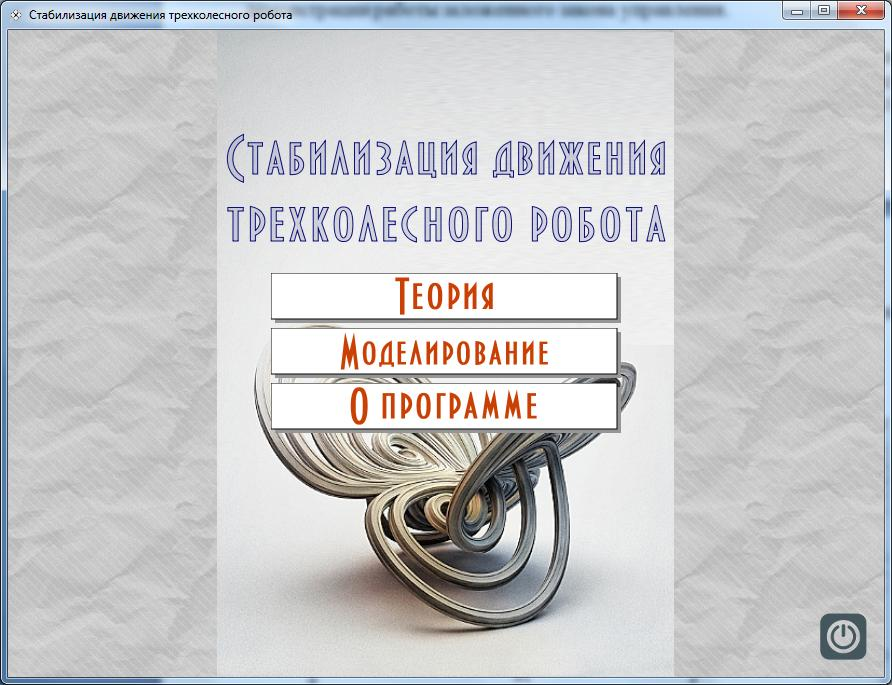
\includegraphics[width=1\linewidth]{window}}
\caption{Основной экран программы}
\label{ris:window}
\end{figure}

\par
\textbf{Теоретический раздел}

В теоретическом разделе содержится схематическое изображение манипулятора, система дифференциальных уравнений, описывающих его движение и краткое теоритеское основание построения управления манипулятором. Подробные теоретические выкладки содержатся в главе 3 настоящей  диссертации.
\nopagebreak[4]
\begin{figure}[h]
\center{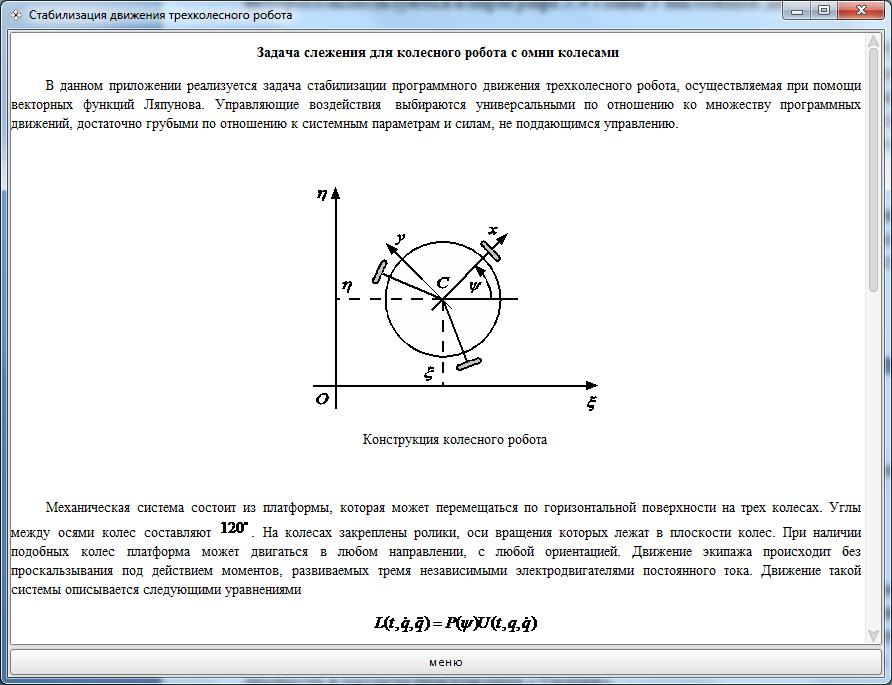
\includegraphics[width=1\linewidth]{theory}}
\caption{Внешний вид теоретического раздела}
\label{ris:theory}
\end{figure} 

\par
\textbf{Раздел моделирование}

В разделе непосредственного моделирования пользователю предлагается задать параметры системы, такие как геометрические характеристики манипулятора (длины звеньев, расстояния до их центров масс), массы звеньев, начальные положения звеньев, а также законы управления в аналитическом виде. Также присутствует возможность автоматического заполенения заранее подобранными значениями по умолчанию для демонстрации работы программы. Значение каждого параметра представлено в теоретическом разделе, на экране моделирования же присутсвуют только сокращенные обозначения, совпадающие с обозначениями в теоретической части.

\begin{figure}[h]
\center{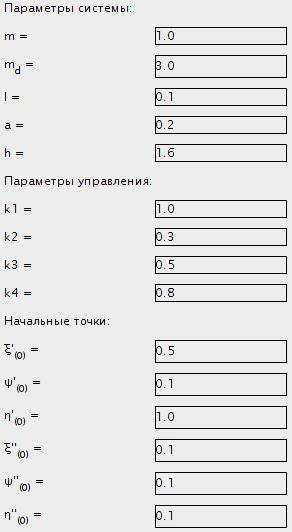
\includegraphics[width=0.5\linewidth]{params}}
\caption{Параметры для расчетов}
\label{ris:params}
\end{figure} 

\begin{figure}[h]
\center{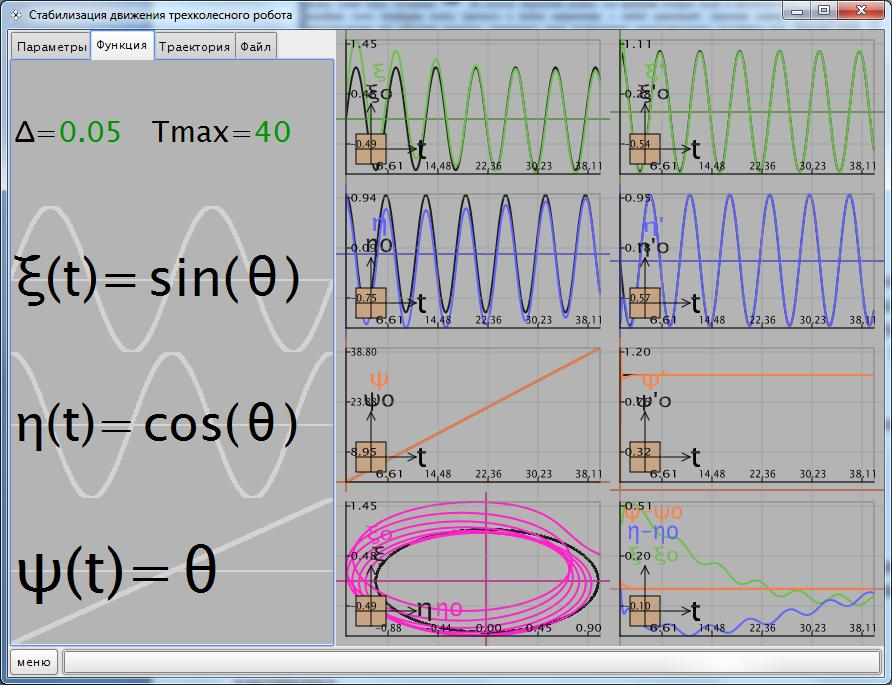
\includegraphics[width=1\linewidth]{modeling}}
\caption{Внешний вид раздела моделирование}
\label{ris:modeling}
\end{figure}

В случае возникновения ошибки, программа сообщает о ней, выделяет незаполненные поля в случае недостаточных данных.
\par
\textbf{Задание закона управления манипулятором аналитически}

Для обработки введенных формул используется открытая сторонняя библиотека, позволяющая пользователю вводить элементарные функции. Также библиотека была доработана для того, чтобы иметь возможность распознавать определенные интегралы с переменным верхним или нижним пределом.

Формулы вводятся в поля ввода в качестве строк текста. В формулах допускается использование констант, основных математических операций и параметров системы, таких, например, как массы звеньев, заданные в виде переменных. При обработке формул происходит преобразование текста в объекты языка Java и сохранение в оперативной памяти. Дальнейшие вычисления проводятся с помощью подстановки вместо переменых констант, необходимых для работы на текущем шаге. Таким образом, обработка формулы производится только на первых шагах, что положительно сказывается на скорости работы программы.

При необходимости библиотке работы с формулами может быть расширена.

Первоначально пользователю предлагается дискретизации $\delta$  и время моделирования  $T_{max}$ рис.\eqref{ris:formul}. После ввода ввода уравнений управления и параметров системы пользователь нажимает на кнопку построения графиков, после чего программа производит моделирование движения манипулятора и отображает результаты в виде графиков, показывающих соответствующее изменение координат каждого из звеньев, а также изменения скоростей звеньев с течением времени, ограничиваясь максимальным временем, заданным пользователем.

\begin{figure}[h]
\center{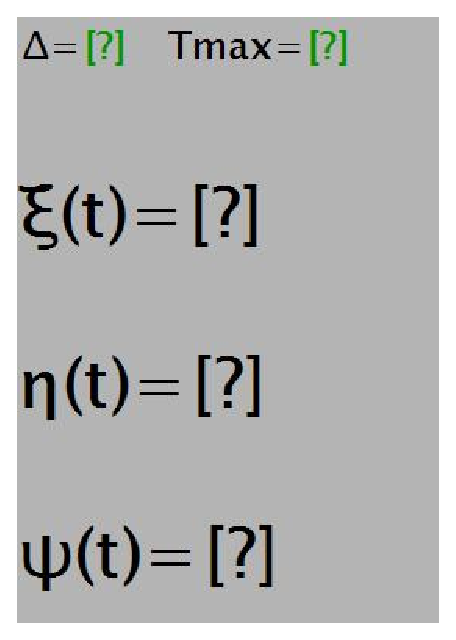
\includegraphics[width=0.5\linewidth]{formul}}
\caption{Система ожидает ввода управления с помощью формул}
\label{ris:formul}
\end{figure}

При наборе формулы поддерживаются следующие действия:
\begin{itemize}
\item{основные математические операции (сложение, вычитание, умножения, деление, возведение в степень);}
\item{ввод формул без ограничения на длину;}
\item{ввод без ограничений по количеству вложенных скобок;}
\item{добавление делегированных тригонометрических и алгебраических функций ($sin(t), cos(t), tg(t), ctg(t), exp(t), ln(t)$ );}
\item{ввод определенных интегралов в том числе с подынтегральной функцией и пределов интегрирования в зависимости от времени $t$;}
\item{ввод независимой переменной $t$;}
\end{itemize}

\textbf{Ввод данных из файла}

При этом вводе данных пользователю необходимо выбрать файл, содержащий заданное управление и параметры системы. В данный момент программой поддерживается два формата хранения данных

\begin{itemize}
\item{cvs;}
\item{json}
\end{itemize}

\begin{figure}[h]
\center{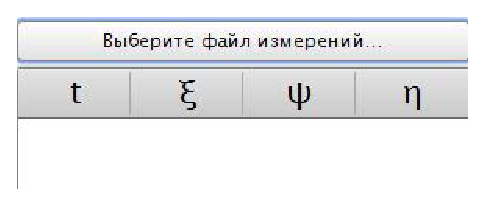
\includegraphics[width=0.5\linewidth]{mass}}
\caption{Внешний вид формы для ввода массива данных}
\label{ris:mass}
\end{figure}

Очередность параметров, считываемых из файла соответсвует порядку их расположения на графическом интерфейсы работы с программой. Так сначала идут параметры системы, затем начальные координаты и скорости звеньев, затем законы управления движением звеньев.

В качества разделителя данных используется символ ";". Дробные числа записываются через символ ".".

\par
\textbf{Расчетная часть}

Для детального ознакомления с реализацией расчета см. Приложение 1.
После задания траектории движения робота одним из описанных способов, в правой части приложения выводятся следующие графики рис.\eqref{ris:graph}

\begin{enumerate}
\item{ графики  $\xi(t), \xi_0(t)$ траектории центра масс платформы }
\item{ графики  $\eta(t), \eta_0(t)$ координаты  центра масс платформы }
\item{ графики  $\psi(t), \psi_0(t)$ угла поворота платформы  }
\item{ графики  $\dot{\xi(t)}, \dot{\xi_0(t)}$ скорости центра масс платформы }
\item{ графики  $\dot{\eta(t)}, \dot{\eta_0(t)}$ скорости координаты  центра масс платформы }
\item{ графики  $\dot{\psi(t)}, \dot{\psi_0(t)}$ скорости поворота платформы  }
\item{ графики траектории платформы  на фазовой плоскости $\xi(\eta(t)), \xi_0(\eta_0(t))$}
\item{ графики  $\|\dot{\xi(t)} - \dot{\xi_0(t)}\|$, $\|\dot{\eta(t)} - \dot{\eta_0(t})\|$, 
$\|\dot{\psi(t)} - \dot{\psi_0(t)}\|$  }
\end{enumerate}
При построении графиков  использовался пятиточечный метод численного дифференцирования.

По графикам можно судить, что рассматриваемая система двигается вдоль отслеживаемой траектории на расстоянии, не превышающем погрешности слежения.

\begin{figure}[h]
\center{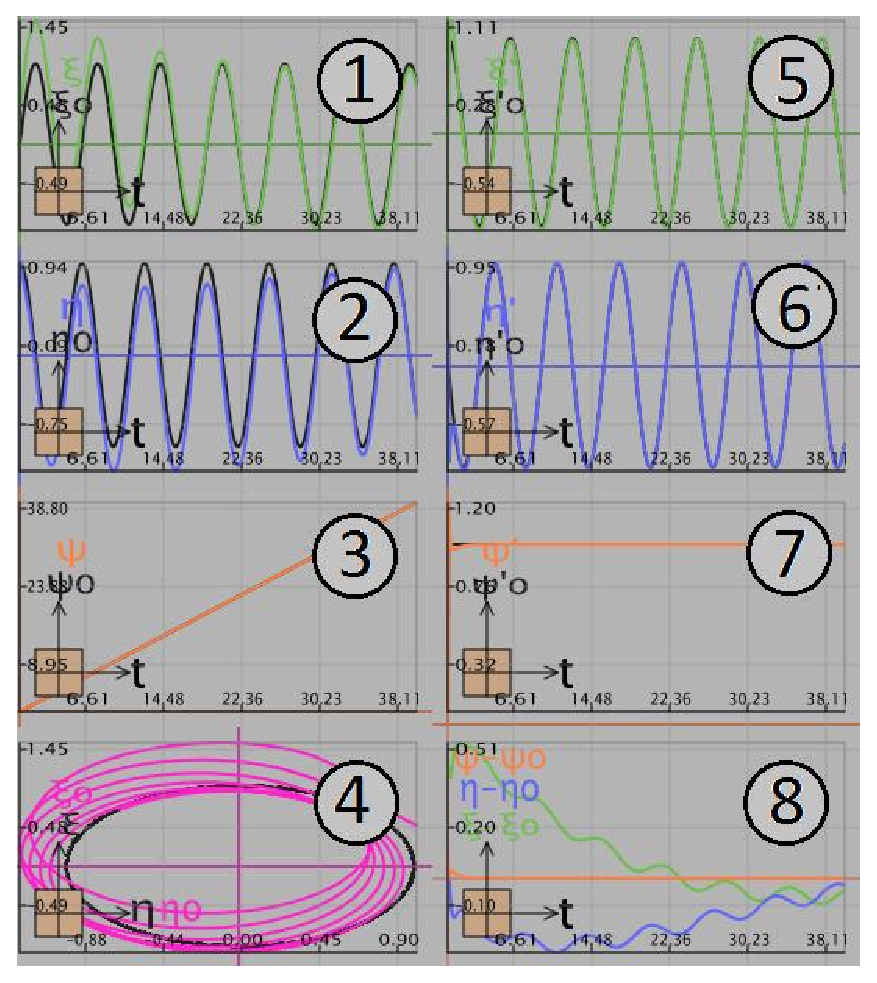
\includegraphics[width=1\linewidth]{graph}}
\caption{Внешний вид расчетной части}
\label{ris:graph}
\end{figure}



\end{document}